%definira klasu dokumenta 
\documentclass[12pt]{report} 

%prostor izmedu naredbi \documentclass i \begin{document} se zove uvod. U njemu se nalaze naredbe koje se odnose na cijeli dokument

%osnovni LaTex ne može riješiti sve probleme, pa se koriste različiti paketi koji olakšavaju izradu željenog dokumenta
\usepackage[croatian]{babel} 
\usepackage{amssymb}
\usepackage{amsmath}
\usepackage{txfonts}
\usepackage{mathdots}
\usepackage{titlesec}
\usepackage{array}
\usepackage{lastpage}
\usepackage{etoolbox}
\usepackage{tabularray}
\usepackage{color, colortbl}
\usepackage{adjustbox}
\usepackage{geometry}
\usepackage[classicReIm]{kpfonts}
\usepackage{hyperref}
\usepackage{fancyhdr}



\usepackage{float}
\usepackage{setspace}
\restylefloat{table}


\patchcmd{\chapter}{\thispagestyle{plain}}{\thispagestyle{fancy}}{}{} %redefiniranje stila stranice u paketu fancyhdr

%oblik naslova poglavlja
\titleformat{\chapter}{\normalfont\huge\bfseries}{\thechapter.}{20pt}{\Huge}
\titlespacing{\chapter}{0pt}{0pt}{40pt}


\linespread{1.3} %razmak između redaka

\geometry{a4paper, left=1in, top=1in,}  %oblik stranice

\hypersetup{ colorlinks, citecolor=black, filecolor=black, linkcolor=black,	urlcolor=black }   %izgled poveznice


%prored smanjen između redaka u nabrajanjima i popisima
\newenvironment{packed_enum}{
	\begin{enumerate}
		\setlength{\itemsep}{0pt}
		\setlength{\parskip}{0pt}
		\setlength{\parsep}{0pt}
	}{\end{enumerate}}

\newenvironment{packed_item}{
	\begin{itemize}
		\setlength{\itemsep}{0pt}
		\setlength{\parskip}{0pt}
		\setlength{\parsep}{0pt}
	}{\end{itemize}}




%boja za privatni i udaljeni kljuc u tablicama
\definecolor{LightBlue}{rgb}{0.9,0.9,1}
\definecolor{LightGreen}{rgb}{0.9,1,0.9}

%Promjena teksta za dugačke tablice
\DefTblrTemplate{contfoot-text}{normal}{Nastavljeno na idućoj stranici}
\SetTblrTemplate{contfoot-text}{normal}
\DefTblrTemplate{conthead-text}{normal}{(Nastavljeno)}
\SetTblrTemplate{conthead-text}{normal}
\DefTblrTemplate{middlehead,lasthead}{normal}{Nastavljeno od prethodne stranice}
\SetTblrTemplate{middlehead,lasthead}{normal}

%podesavanje zaglavlja i podnožja

\pagestyle{fancy}
\lhead{Programsko inženjerstvo}
\rhead{IznajmiRomobil}
\lfoot{ScootShare}
\cfoot{stranica \thepage/\pageref{LastPage}}
\rfoot{\today}
\renewcommand{\headrulewidth}{0.2pt}
\renewcommand{\footrulewidth}{0.2pt}


\begin{document} 
	
	
	
	\begin{titlepage}
		\begin{center}
			\vspace*{\stretch{1.0}} %u kombinaciji s ostalim \vspace naredbama definira razmak između redaka teksta
			\LARGE Programsko inženjerstvo\\
			\large Ak. god. 2023./2024.\\
			
			\vspace*{\stretch{3.0}}
			
			\huge Iznajmi Romobil\\
			\Large Dokumentacija, Rev. \textit{1}\\
			
			\vspace*{\stretch{12.0}}
			\normalsize
			Grupa: \textit{ScootShare}\\
			Voditelj: \textit{Ivan Pavelić}\\
			
			
			\vspace*{\stretch{1.0}}
			Datum predaje: \textit{$17$. $11$. $2023$.}\\
	
			\vspace*{\stretch{4.0}}
			
			Nastavnik: \textit{Igor Stančin}\\
		
		\end{center}

	
	\end{titlepage}

	
	\tableofcontents


	\chapter{Dnevnik promjena dokumentacije}
		
				
		
		\begin{longtblr}[
				label=none
			]{
				width = \textwidth, 
				colspec={|X[2]|X[13]|X[3]|X[3]|}, 
				rowhead = 1
			}
			\hline
			\textbf{Rev.}	& \textbf{Opis promjene/dodatka} & \textbf{Autori} & \textbf{Datum}\\[3pt] \hline
			0.1 & Napravljen predložak.	& Karmen Korić, Dino Babić, Jan Grbac, Anamarija Jakoubek, Ivan Pavelić, Igor Šoštarko, Leonarda Pribanić & 20.10.2023. 		\\[3pt] \hline 
			0.2	& Dopisane upute za povijest dokumentacije.\newline Dodane reference. & * & 24.08.2013. 	\\[3pt] \hline 
			0.5 & Dodan \textit{Use Case} dijagram i jedan sekvencijski dijagram, funkcionalni i nefunkcionalni zahtjevi i dodatak A & * & 25.08.2013. \\[3pt] \hline 
			0.6 & Arhitektura i dizajn sustava, algoritmi i strukture podataka & * & 26.08.2013. \\[3pt] \hline 
			0.8 & Povijest rada i trenutni status implementacije,\newline Zaključci i plan daljnjeg rada & * & 28.08.2013. \\[3pt] \hline 
			0.9 & Opisi obrazaca uporabe & * & 07.09.2013. \\[3pt] \hline 
			0.10 & Preveden uvod & * & 08.09.2013. \\[3pt] \hline 
			0.11 & Sekvencijski dijagrami & * & 09.09.2013. \\[3pt] \hline 
			0.12.1 & Započeo dijagrame razreda & * & 10.09.2013. \\[3pt] \hline 
			0.12.2 & Nastavak dijagrama razreda & * & 11.09.2013. \\[3pt] \hline 
			\textbf{1.0} & Verzija samo s bitnim dijelovima za 1. ciklus & * & 11.09.2013. \\[3pt] \hline 
		\end{longtblr}
	
	\chapter{Opis projektnog zadatka}
		
		\indent Cilj ovog projekta je razviti programsku podršku za stvaranje web aplikacije \emph{"Iznajmi Romobil"} koja će korisniku omogućiti da iznajmi vlastiti romobil u vrijeme kada ga ne koristi, a korisnicima koji ne posjeduju romobil daje mogućost najma romobila. \newline
		\indent Prilikom pokretanja aplikacije prikazuje se glavna stranica s oglasima za najam romobila. Neprijvljen korisnik oglase može samo pregledavati, dok prijavljen korisnik može i stupiti u kontakt s iznajmljivačem te u konačnici i unajmiti odabrani romobil. \\
		\indent Ako korisnik nema izrađen račun u aplikaciji, ima mogućnost registracije. Prilikom registracije, korisnik unosi:
		\begin{packed_item} 
			\item {ime}
			\item {prezime}
			\item {nadimak}
			\item {email adresa}
			\item {broj kartice}
			\item {korisničko ime}
			\item {lozinka}
			\item {kopija osobne iskaznice}
			\item {potvrda o nekažnjavanju}  
		\end{packed_item}
		\indent Tijekom obrade registracije na strani poslužitelja korisniku se dodijeljuju ovlasti. S obzirom na to da korisnik može biti i iznajmljivač i klijent, jedna će ovlast  objediniti te uloge. Također, sustav razlikuje i ovlast admin.  \\
		\indent Jednom kada se korisnik registrira, ili je već prije izradio račun, ima mogućnost prijave u aplikaciju. Prilikom prijave korisnik unosi korisničko ime i lozinku. Jednom kada potvrdi prijavu, na poslužiteljsku stranu šalju se uneseni podaci, a povratno poslužitelj odgovara ili s greškom ili s JSON web tokenom u kojem su spremljeni korisničko ime i njegove ovlasti.
		\indent Ako je prijava uspješno provedena korisnika se proslieđuje na početnu stranicu. Kao što je prethodno navedeno, prijavljeni korisnik sada može iznajmljivati i unajmljivati romobile. Da bi iznajmljivač postavio svoj romobil na iznajmljivanje mora ga registrirat. Prilikom registracije romobila iznajmljivač unosi slike romobila kao dokaz trenutnog stanja. Jednom kada je romobil registriran, iznajmljivač postavlja ponude za iznajmljivanje te za svaku unosi:
		\begin{packed_item} 
			\item trenutna lokacija romobila
			\item lokacija povratka romobila
			\item vrijeme povratka romobila
			\item cijena iznajmljivanja po prijeđenom kilometru
			\item iznos novčane kazne u slučaju da romobil ne bude vraćen na vrijeme
		\end{packed_item}
		Iznajmljivač svoju ponudu može objaviti i na društvenoj mreži Facebook.\\
		\indent Klijent pretražuje oglase i kada se odluči za romobil, može se javiti iznajmljivaču. Komunikacija između klijenta i iznajmljivača odvija se preko poruka putem aplikacije. Iznajmljivač i klijent mogu razmijeniti o vremenu preuzimanja, samom romobilu i tomu slično. Ako stvarno stanje romobila kojeg klijent preuzme ne odgovara stanju kakvo je prikazano na slikama, klijent može stare slike romobila zamijeniti vlastitim. Također, može i dati kratki opis razlika između starih slika i stvarnog stanja. Ako iznajmljivač smatra da zamjena slika nije utemeljena, tu zamjenu može prijaviti administratoru. Klijent je dužan vratiti romobila u zadano vrijeme i lokaciju povratka.  \\
		\indent Admin je korisnik najveće razine te on ima mogućnost pregleda svih korisnika i može ih brisati. Admin pregledava prijave iznajmljivača i odlučuje hoće li se zamjena slika izvršiti i li ne. Njegova odluka dolazi kao obavijest klijentu i iznajmljivaču. Također, admin pregledava dostavljenu kopiju osobne iskaznice i potvrdu o nekažnjavanju. Ako uspostavi da su dokumenti neispravni, može trajno ukolniti korisnika s aplikacije.\\
		\indent Mjerač prijeđenih kilometara na romobilima i aplikacija su povezani. Kada istekne vrijeme povratka iznajmljivač dobiva obavijest u aplikaciji u kojoj je navedeno koliko je kilometara klijent prešao. Klijent također dobiva obavijest u kojoj su napisani detalji transakcije. \\
		\indent Nakon što je iznajmljivanje završeno, iznajmljivač može ocijeniti klijenta i napisati komentar. Ocjene i komentari su vidljivi na profilima korisnika. \\
		\indent Korisnik na svom profilu može pregledati podatke o prethodnim vožnjama, ili ako se radi o iznajmljivaču podatke o prethodnim najmovima romobila.\\ \\
		
		\indent Korist ovog projekta je omogućiti ljudima jednostavan pristup električnim romobilima. Kvalitetan električni romobil je mnogima preskup, tako da oni koji ga ne posjeduju mogu lako i brzo iznajmiti romobil na dane kada im je potreban. Ljudi koji ne koriste svoj romobil, a ne žele da propada u skladišu, mogu ga iznajmiti drugima i na taj način ostvariti dodatan prihod. \\
		\indent U urbanim sredinama gužve u prometu postaju sveprisutni problem koji otežava svakodnevno kretanje i troši vrijeme. U takvim okolnostima, ljudi traže alternativne metode prijevoza koje su brže, praktičnije i održive. I tu vidimo prilku za našu aplikaciju.\\
		\indent Aplikacija bi mogla biti unaprijeđena tako da klijent ima veću mogućnost filtriranja prikazanih oglasa. Na primjer može pretraživati oglase samo u okolici njegove lokacije ili romobile koji zadovoljavaju njegove zahtjeve, na primjer da maksimalna brzina romobila nije manja od 45km/h i tomu slično. \\
		
		\indent Tvrtka Bolt, koja je u hrvatskoj prepoznatljiva po uslugama dostave hrane i prijevoza, u pojedinim gradovima nudi mogućnost najma romobila. Pa se tako u glavnom gradu Belgije, Brisselu, romobili spremni za najam mogu pronaći gotovo u svakoj ulici. Potrebno je imati novčana sredstva u Bolt aplikaciji, na romobilu se skenira QR kod i spremni ste za vožnju. Cijena se također obračunava po prijeđenom kilometru. A jednom kada ste gotovi odjavite se s romobila, romobil se zaključa i spreman je za idućeg korisnika, a Vama se automatksi provede transakcija.
		
		
		\begin{figure}[h]
			\centering
			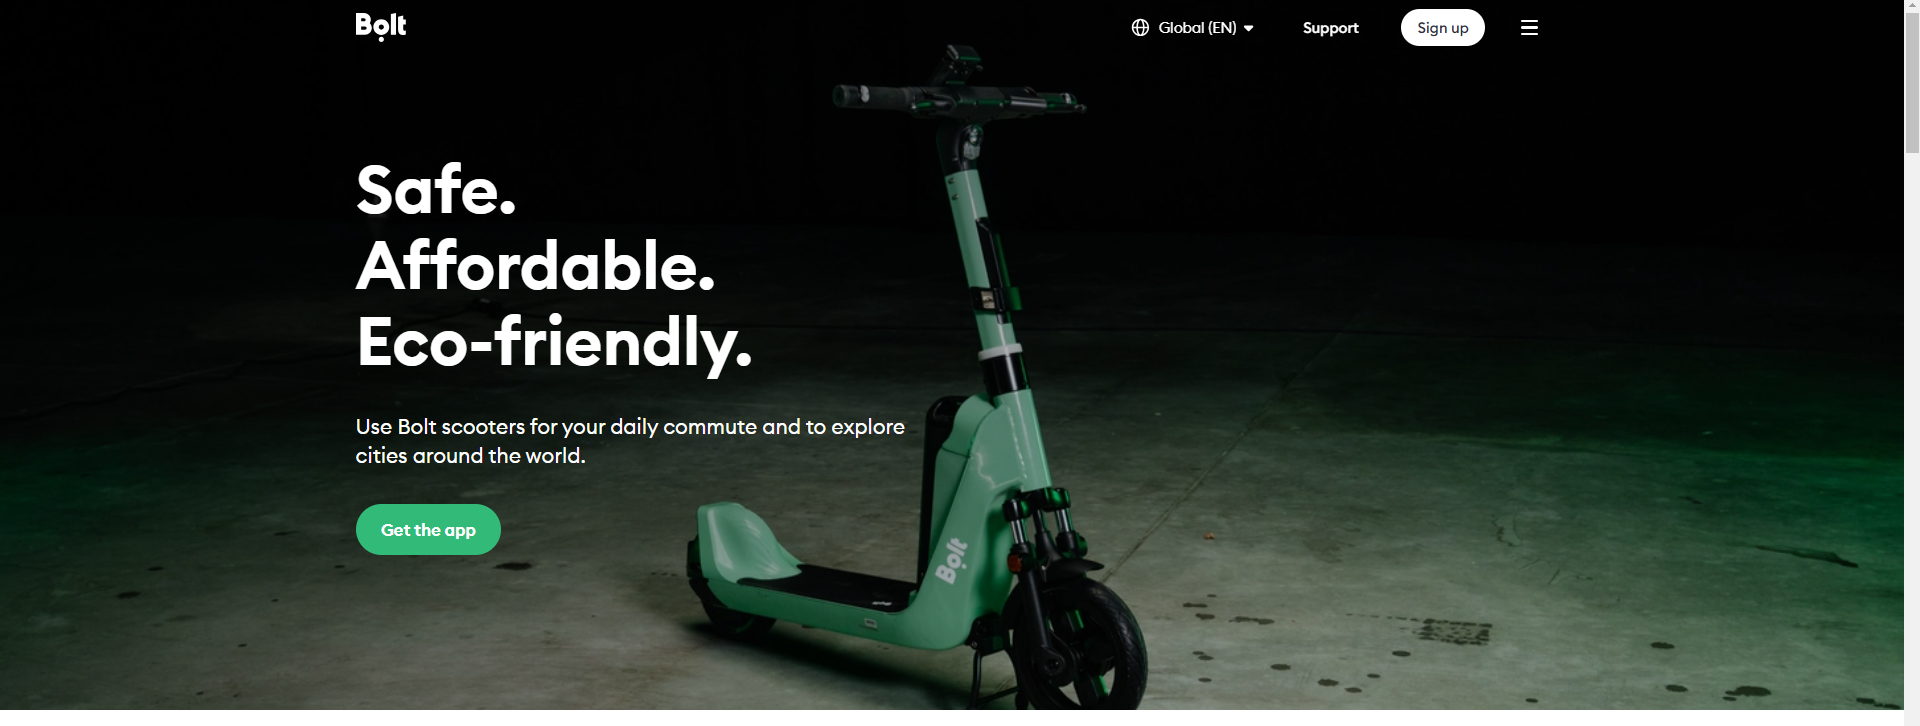
\includegraphics[width=0.8\textwidth]{bolt-1.png}
			\caption{Početna stranica za najam rombila tvrtke Bolt}
			\label{fig:your_label}
		\end{figure}
		
		\begin{figure}[t]
			\centering
			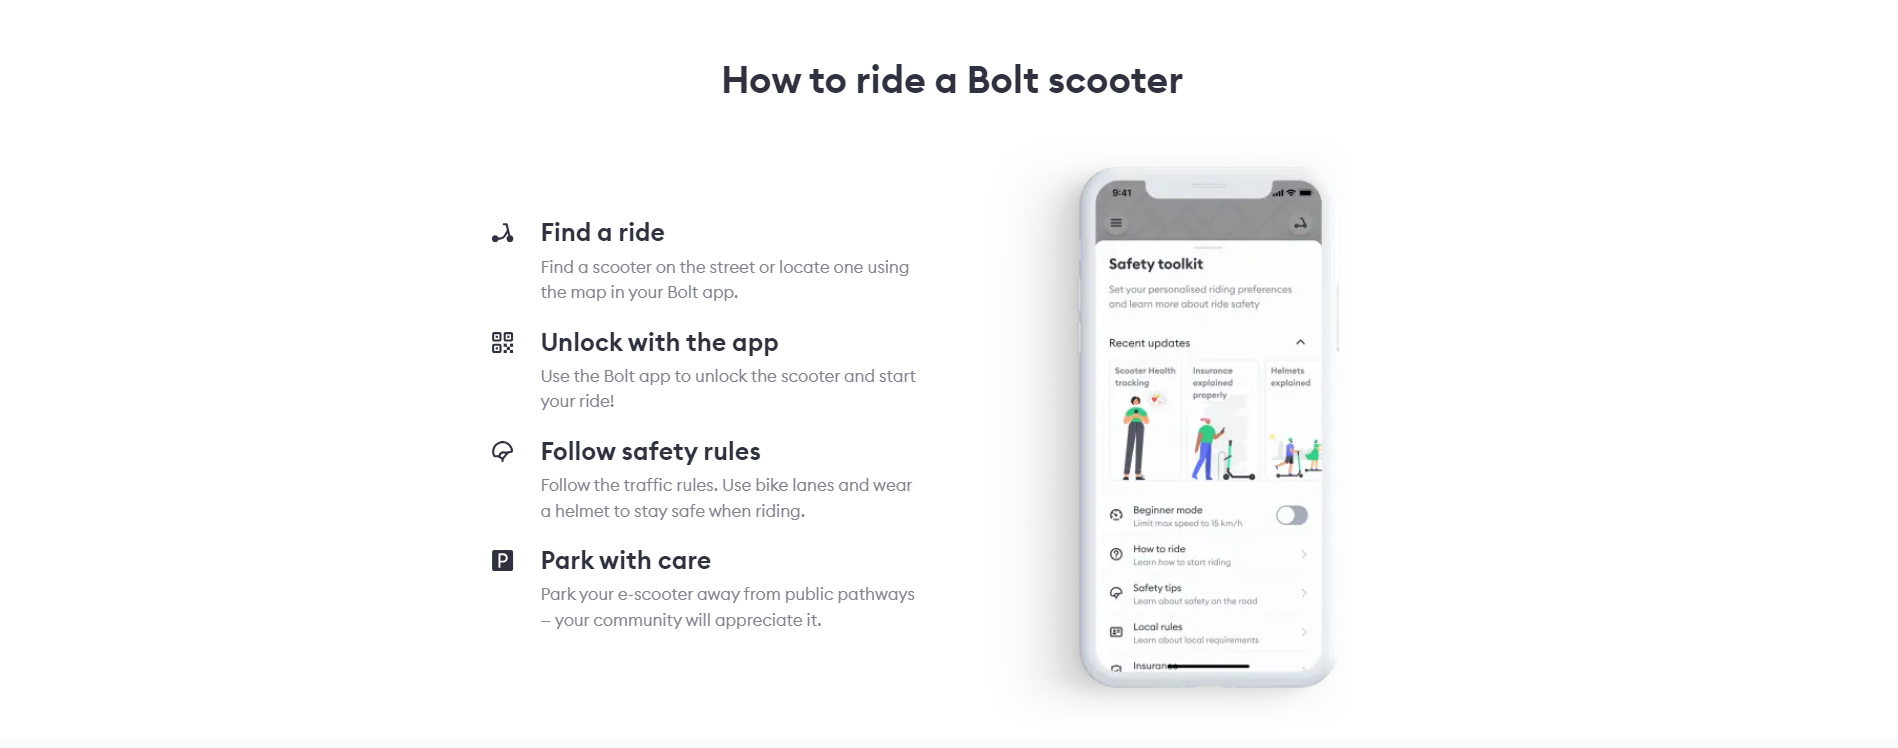
\includegraphics[width=0.8\textwidth]{bolt-2.png}
			\caption{Instrukcije za korištenje romobila tvrtke Bolt}
			\label{fig:your_label}
		\end{figure}
		
		\indent Aplikacija Fat LIama nudi mogućnost najma električnih romobila diljem svijeta. Razlikuje se po tome što je cijena iskazana po danu najma. Korisnik može odabrati lokaciju, pretražuje ponuđene oglase te ima mogućnost najma na više dana.\\
		 
		 \begin{figure}[t]
		 	\centering
		 	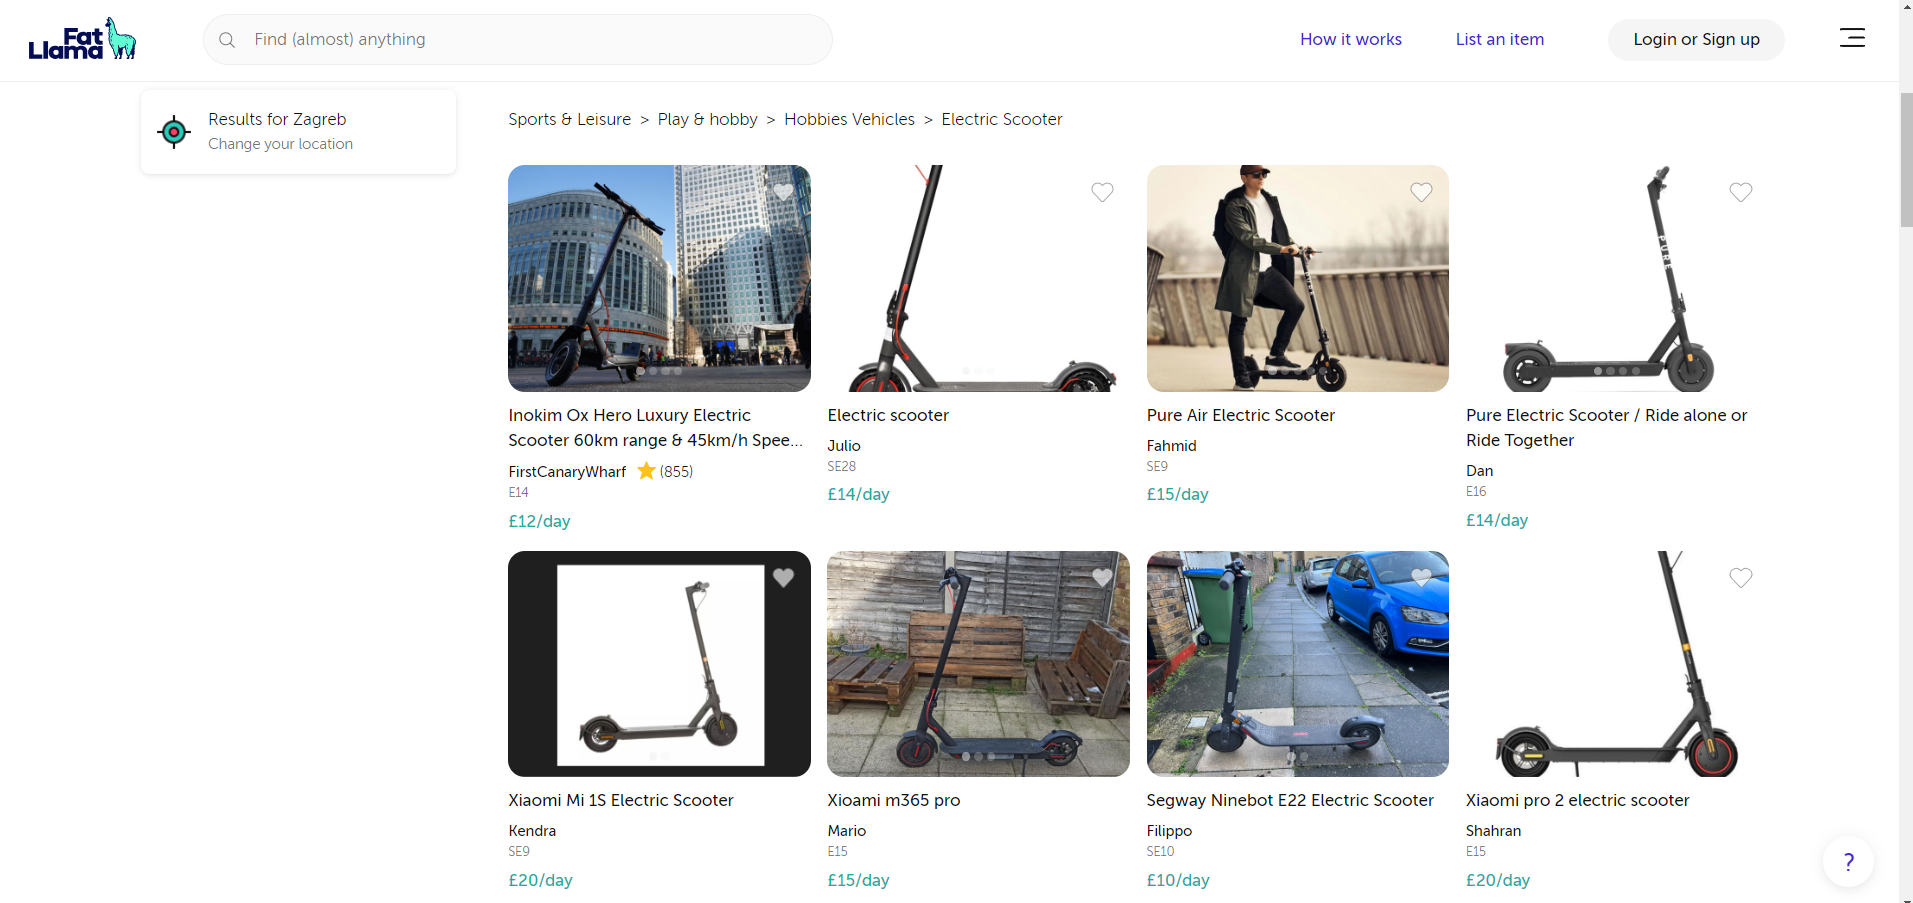
\includegraphics[width=0.8\textwidth]{fat-liama.png}
		 	\caption{Najam romobila Fat LIama}
		 	\label{fig:your_label}
		 \end{figure}
		
		
		
		
	
	\chapter{Specifikacija programske potpore}
		
	\section{Funkcionalni zahtjevi}
			
			
			
			\noindent \textbf{Dionici:}
			
			\begin{packed_enum}
				
				\item Neregistrirani korisnik
				\item Prijavljeni korisnik
				\item Klijent				
				\item Iznajmljivač
				\item Administrator

				
			\end{packed_enum}
			
			\noindent \textbf{Aktori i njihovi funkcionalni zahtjevi:}
			


			\begin{packed_enum}

				\item  \underbar{Neregistrirani korisnik može: }
				
				\begin{packed_enum}
					
					\item se registrirati u sustav, stvoriti novi korisnički račun sa svim potrebnim podatcima
					\item pregledavati trenutno dostupne romobile i njihove cijene

				\end{packed_enum}

				\item  \underbar{Prijavljeni korisnik može: }
				
				\begin{packed_enum}
					
					\item prijaviti se s postojećim podacima za prijavu u sustav
					\item pregledavati dostupne romobile
					\item upravljati svojim osobnim podatcima
					\item pregledati povijest svojih transakcija


				\end{packed_enum}
			
				\item  \underbar{Klijent može:}
				
				\begin{packed_enum}
					
					\item iznajmljivati dostupne romobile te provjeriti je li slike odgovaraju stvarnom stanju
					\item zamijeniti sliku koja ne odgovara stvarnom stanju iznajmljenog romobila novom slikom i kratkim opisom
					\item javiti se iznajmljivaču s porukom i zahtjevom za iznajmljivanje
					
				\end{packed_enum}

				\item  \underbar{Iznajmljivač može: }
				
				\begin{packed_enum}
					
					\item registrirati romobil za što su mu potrebne slike romobila kao dokaz trenutnog stanja
					\item postaviti ponudu za iznajmljivanje i pritom mora unijeti sve relevantne podatke
					\item objaviti na društvenoj mreži o dostupnosti romobila za iznajmljivanje
					\item prijaviti administratoru ako je zamjena slika iznajmljenog romobila predložena bez dobrog razloga
					\item odgovoriti klijentu i prihvatiti ili odbiti ponudu
					\item ocijeniti klijenta i napisati komentar

				\end{packed_enum}

				\item  \underbar{Administrator može: }
				
				\begin{packed_enum}
					
					\item pregledava prijave iznajmljivača i odlučuje hoće li se zamjena slika izvršiti ili ne
					\item pregledava dokumente poslane prilikom registracije te registraciju odobrava ili odbija
					\item zabraniti pristupa svim korisnicima

				\end{packed_enum}

				\item  \underbar{Baza podataka (sudionik) može: }
				
				\begin{packed_enum}
					
					\item pohranjuje sve podatke o korisnicima i njihovim romobilima
					\item pohranjuje sve podatke o transakcijama

				\end{packed_enum}
			\end{packed_enum}
			
			\eject 
			
			
				
			\subsection{Obrasci uporabe}

				
				\subsubsection{Opis obrazaca uporabe}

					

					\noindent \underbar{\textbf{UC1 - Pregled romobila}}
					\begin{packed_item}
	
						\item \textbf{Glavni sudionik: }Prijavljeni korisnik
						\item  \textbf{Cilj: }Pregledati romobile i njihove cijene
						\item  \textbf{Sudionici: }Baza podataka
						\item  \textbf{Preduvjet: }-
						\item  \textbf{Opis osnovnog tijeka:}
						
						\item[] \begin{packed_enum}
	
							\item Prikazani su dostupni romobili
							\item Korisnik odabire romobil
							\item Prikazuju se informacije i slike romobila te uvjeti za iznajmljivanje

						\end{packed_enum}
					\end{packed_item}
						
					

					\noindent \underbar{\textbf{UC2 - Registracija}}
					\begin{packed_item}
	
						\item \textbf{Glavni sudionik: }Neregistrirani korisnik
						\item  \textbf{Cilj: }Stvoriti korisnički račun za pristup sustavu
						\item  \textbf{Sudionici: }Baza podataka
						\item  \textbf{Preduvjet: }-
						\item  \textbf{Opis osnovnog tijeka:}
						
						\item[] \begin{packed_enum}
	
							\item Korisnik odabire opciju za registraciju
							\item Korisnik unosi potrebne korisničke podatke
							\item Sustav provjerava ispravnost podataka
							\item Korisnik prima obavijest o uspješnoj registraciji
							\item Sustav preusmjerava korisnika na stranicu s aktivnim oglasima

						\end{packed_enum}
						
						\item  \textbf{Opis mogućih odstupanja:}
						
						\item[] \begin{packed_item}
	
							\item[2.a] Odabir već zauzetog e-maila, unos korisničkog podatka u nedozvoljenom formatu
							\item[] \begin{packed_enum}
								
								\item Sustav obavještava korisnika o neuspjelom pokušaju registracije i vraća ga na stranicu za registraciju
								\item Korisnik mijenja potrebne podatke te završava registraciju ili odustaje od nje
								
							\end{packed_enum}
							
						\end{packed_item}						
					\end{packed_item}



						\noindent \underbar{\textbf{UC3 - Prijava u sustav}}
					\begin{packed_item}
	
						\item \textbf{Glavni sudionik: }Prijavljeni korisnik
						\item  \textbf{Cilj: }Dobiti pristup korisničkom sučelju
						\item  \textbf{Sudionici: }Baza podataka
						\item  \textbf{Preduvjet: }Registracija
						\item  \textbf{Opis osnovnog tijeka:}
						
						\item[] \begin{packed_enum}
	
							\item Korisnik odabire opciju za prijavu
							\item Korisnik unosi potrebne korisničke podatke
							\item Sustav provjerava ispravnost podataka
							\item Pristup korisničkim funkcijama

						\end{packed_enum}
						
						\item  \textbf{Opis mogućih odstupanja:}
						
						\item[] \begin{packed_item}
	
							\item[2.a] Neispravni korisnički podatci
							\item[] \begin{packed_enum}
								
								\item Sustav obavještava korisnika o neuspjelom pokušaju prijave i vraća ga na stranicu za prijavu
								
							\end{packed_enum}
							
						\end{packed_item}						
					\end{packed_item}			
					



						\noindent \underbar{\textbf{UC4 - Pregled dokumenata poslanih prilikom registracije}}
					\begin{packed_item}
	
						\item \textbf{Glavni sudionik: }Administrator
						\item  \textbf{Cilj: }Odobravanje ili odbijanje registracije
						\item  \textbf{Sudionici: }Baza podataka
						\item  \textbf{Preduvjet: }Administrator je prijavljen i novi korisnik je registriran
						\item  \textbf{Opis osnovnog tijeka:}
						
						\item[] \begin{packed_enum}
	
							\item Administrator pregledava dokumente poslane prilikom registracije
							\item Registraciju odobrava ili odbija
							\item Odluka dolazi kao obavijest korisniku

						\end{packed_enum}					
					\end{packed_item}	



						\noindent \underbar{\textbf{UC5 - Pregled osobnih podataka}}
					\begin{packed_item}
	
						\item \textbf{Glavni sudionik: }Prijavljeni korisnik
						\item  \textbf{Cilj: }Pregledati osobne podatke
						\item  \textbf{Sudionici: }Baza podataka
						\item  \textbf{Preduvjet: }Korisnik je prijavljen
						\item  \textbf{Opis osnovnog tijeka:}
						
						\item[] \begin{packed_enum}
	
							\item Korisnik odabire opciju za pregled svojih podataka
							\item Aplikacija prikazuje osobne podatke korisnika

						\end{packed_enum}					
					\end{packed_item}	


						\noindent \underbar{\textbf{UC6 - Promjena osobnih podataka}}
					\begin{packed_item}
	
						\item \textbf{Glavni sudionik: }Prijavljeni korisnik
						\item  \textbf{Cilj: }Promijeniti osobne podatke
						\item  \textbf{Sudionici: }Baza podataka
						\item  \textbf{Preduvjet: }Korisnik je prijavljen
						\item  \textbf{Opis osnovnog tijeka:}
						
						\item[] \begin{packed_enum}
	
							\item Korisnik odabire opciju za pregled svojih podataka
							\item Korisnik odabere opciju za promjenu podataka
							\item Korisnik mijenja svoje osobne podatke
							\item Korisnik sprema promjene
							\item Baza podataka se ažurira


						\end{packed_enum}
						
						\item  \textbf{Opis mogućih odstupanja:}
						
						\item[] \begin{packed_item}
	
							\item[3.a] Neki podatci nisu popunjeni
							\item[] \begin{packed_enum}
								
								\item Sustav javlja da nisu uneseni svi potrebni podaci
								\item Korisnik dodaje potrebne podatke te završava promjenu ili odustaje od nje
								
							\end{packed_enum}
							
						\end{packed_item}						
					\end{packed_item}	


						\noindent \underbar{\textbf{UC7 - Registriranje romobila}}
					\begin{packed_item}
	
						\item \textbf{Glavni sudionik: }Iznajmljivač
						\item  \textbf{Cilj: }Registracija novog romobila
						\item  \textbf{Sudionici: }Baza podataka
						\item  \textbf{Preduvjet: }Korisnik je prijavljen
						\item  \textbf{Opis osnovnog tijeka:}
						
						\item[] \begin{packed_enum}
	
							\item Korisnik odabire opciju za registriranje romobila
							\item Korisnik popunjava tražena podatke
							\item Korisnik sprema promjene
							\item Baza se ažurira


						\end{packed_enum}
						
						\item  \textbf{Opis mogućih odstupanja:}
						
						\item[] \begin{packed_item}
	
							\item[2.a] Nisu popunjena sva polja obrasca
							\item[] \begin{packed_enum}
								
								\item Sustav javlja da nisu uneseni svi podaci
								\item Korisnik dodaje potrebne podatke te završava registraciju ili odustaje od nje

								
							\end{packed_enum}
							
						\end{packed_item}						
					\end{packed_item}	






						\noindent \underbar{\textbf{UC8 - Postavljanje ponude za iznajmljivanje}}
					\begin{packed_item}
	
						\item \textbf{Glavni sudionik: }Iznajmljivač
						\item  \textbf{Cilj: }Stvoriti novu ponudu za iznajmljivanje romobila
						\item  \textbf{Sudionici: }Baza podataka
						\item  \textbf{Preduvjet: }Korisnik je prijavljen i romobil je registriran
						\item  \textbf{Opis osnovnog tijeka:}
						
						\item[] \begin{packed_enum}
	
							\item Korisnik odabire opciju za stvaranje nove ponude
							\item Korisnik popunjava potrebne podatke
							\item Korisnik sprema promjene
							\item Baza se ažurira


						\end{packed_enum}
						
						\item  \textbf{Opis mogućih odstupanja:}
						
						\item[] \begin{packed_item}
	
							\item[2.a] Nisu popunjena sva polja obrasca
							\item[] \begin{packed_enum}
								
								\item Sustav javlja da nisu uneseni svi podaci
								\item Korisnik dodaje potrebne podatke te završava ponudu ili odustaje od nje

								
							\end{packed_enum}
							
						\end{packed_item}						
					\end{packed_item}	





						\noindent \underbar{\textbf{UC9 - Objavljivanje ponude na društvenoj mreži}}
					\begin{packed_item}
	
						\item \textbf{Glavni sudionik: }Iznajmljivač
						\item  \textbf{Cilj: }Objava na društvenoj mreži o dostupnosti romobila za iznajmljivanje
						\item  \textbf{Sudionici: }Baza podataka
						\item  \textbf{Preduvjet: }Korisnik je prijavljen i postoji ponuda za iznajmljivanje
						\item  \textbf{Opis osnovnog tijeka:}
						
						\item[] \begin{packed_enum}
	
							\item Korisnik odabire oglas
							\item Korisnik objavljuje na društvenoj mreži o dostupnosti romobila za iznajmljivanje


						\end{packed_enum}						
					\end{packed_item}	



						\noindent \underbar{\textbf{UC10 - Kontaktiranje iznajmljivača}}
					\begin{packed_item}
	
						\item \textbf{Glavni sudionik: }Klijent
						\item  \textbf{Cilj: }Podnošenje zahtjeva za iznajmljivanje romobila
						\item  \textbf{Sudionici: }Baza podataka
						\item  \textbf{Preduvjet: }Klijent je prijavljen i postoji romobil za iznajmljivanje
						\item  \textbf{Opis osnovnog tijeka:}
						
						\item[] \begin{packed_enum}
	
							\item Klijent odabire romobil koji želi iznajmit
							\item Klijent se javlja iznajmljivaču s porukom i zahtjevom za iznajmljivanje


						\end{packed_enum}						
					\end{packed_item}	




						\noindent \underbar{\textbf{UC11 - Prihvaćanje ponude}}
					\begin{packed_item}
	
						\item \textbf{Glavni sudionik: }Iznajmljivač
						\item  \textbf{Cilj: }Odluka o iznajmljivanju romobila
						\item  \textbf{Sudionici: }Baza podataka
						\item  \textbf{Preduvjet: }Iznajmljivač je prijavljen i postoji zahtjev za iznajmljivanje
						\item  \textbf{Opis osnovnog tijeka:}
						
						\item[] \begin{packed_enum}
	
							\item Iznajmljivač pregledava zahtjev za iznajmljivanje romobila
							\item Iznajmljivač ga prihvaća ili odbija
							\item Odluka dolazi kao obavijest klijentu


						\end{packed_enum}						
					\end{packed_item}	



						\noindent \underbar{\textbf{UC12 - Iznajmljivanje romobila}}
					\begin{packed_item}
	
						\item \textbf{Glavni sudionik: }Klijent
						\item  \textbf{Cilj: }Najam romobila i provjera odgovaraju li slike romobila stvarnom stanju
						\item  \textbf{Sudionici: }Baza podataka, iznajmljivač
						\item  \textbf{Preduvjet: }Klijent je prijavljen i iznajmljivač je potvrdio zahtjev
						\item  \textbf{Opis osnovnog tijeka:}
						
						\item[] \begin{packed_enum}
	
							\item Klijent izvršava plaćanje 
							\item Klijent provjerava je li romobil odgovara slikama iz ponude


						\end{packed_enum}						
					\end{packed_item}	




						\noindent \underbar{\textbf{UC13 - Zamjena slike romobila}}
					\begin{packed_item}
	
						\item \textbf{Glavni sudionik: }Klijent
						\item  \textbf{Cilj: }Zamjena neodgovarajuće slike romobila sa novom slikom i kratkim opisom što je drugačije na slici
						\item  \textbf{Sudionici: }Baza podataka
						\item  \textbf{Preduvjet: }Klijent je prijavljen i iznajmio je romobil
						\item  \textbf{Opis osnovnog tijeka:}
						
						\item[] \begin{packed_enum}
	
							\item Klijent odabire sliku koju želi zamijeniti
							\item Klijent učitava novu sliku i opis što je drugačije
							\item Klijent sprema promjene
							\item Baza se ažurira


						\end{packed_enum}
						
						\item  \textbf{Opis mogućih odstupanja:}
						
						\item[] \begin{packed_item}
	
							\item[2.a] Nisu popunjena sva polja
							\item[] \begin{packed_enum}
								
								\item Sustav javlja da nisu uneseni svi podaci
								\item Korisnik dodaje potrebne podatke te završava zamjenu ili odustaje od nje

							\end{packed_enum}
							
						\end{packed_item}						
					\end{packed_item}	




						\noindent \underbar{\textbf{UC14 - Prijava pogrešne zamjene}}
					\begin{packed_item}
	
						\item \textbf{Glavni sudionik: }Iznajmljivač
						\item  \textbf{Cilj: }Prijava administratoru da je zamjena slika predložena bez dobrog razloga
						\item  \textbf{Sudionici: }Baza podataka
						\item  \textbf{Preduvjet: }Iznajmljivač je prijavljen i romobil je iznajmljen, izvršena je zamjena slika od strane klijenta
						\item  \textbf{Opis osnovnog tijeka:}
						
						\item[] \begin{packed_enum}
	
							\item Klijent odabire promijenjenu sliku
							\item Klijent odabire prijavu zamjene s kratkim opisom
							\item Klijent sprema promjene
							\item Baza se ažurira


						\end{packed_enum}
						
						\item  \textbf{Opis mogućih odstupanja:}
						
						\item[] \begin{packed_item}
	
							\item[2.a] Nisu popunjena sva polja
							\item[] \begin{packed_enum}
								
								\item Sustav javlja da nisu uneseni svi podaci
								\item Korisnik dodaje potrebne podatke te završava prijavu ili odustaje od nje

							\end{packed_enum}
							
						\end{packed_item}						
					\end{packed_item}	






						\noindent \underbar{\textbf{UC15 - Pregled prijave}}
					\begin{packed_item}
	
						\item \textbf{Glavni sudionik: }Administrator
						\item  \textbf{Cilj: }Odluka o zamjeni slika
						\item  \textbf{Sudionici: }Baza podataka
						\item  \textbf{Preduvjet: }Administrator je prijavljen i podnesena je prijava zamjene slika
						\item  \textbf{Opis osnovnog tijeka:}
						
						\item[] \begin{packed_enum}
	
							\item Administrator pregledava prijave iznajmljivača
							\item Donosi odluku hoće li se zamjena slika izvršiti ili ne
							\item Odluka dolazi kao obavijest i klijentu i iznajmljivaču
							\item Baza se ažurira


						\end{packed_enum}
									
					\end{packed_item}	





						\noindent \underbar{\textbf{UC16 - Ocjenjivanje klijenta}}
					\begin{packed_item}
	
						\item \textbf{Glavni sudionik: }Iznajmljivač
						\item  \textbf{Cilj: }Ocjena klijenta i objava komentara
						\item  \textbf{Sudionici: }Baza podataka
						\item  \textbf{Preduvjet: }Iznajmljivač je prijavljen i romobil je iznajmljen
						\item  \textbf{Opis osnovnog tijeka:}
						
						\item[] \begin{packed_enum}
	
							\item Iznajmljivač odabire klijenta
							\item Dodjeljuje mu ocjenu i piše komentar
							\item Ocjena i komentar se objavljuju na profilu.
							\item Baza se ažurira


						\end{packed_enum}
						
						\item  \textbf{Opis mogućih odstupanja:}
						
						\item[] \begin{packed_item}
	
							\item[2.a] Nisu popunjena sva polja
							\item[] \begin{packed_enum}
								
								\item Sustav javlja da nisu uneseni svi podaci
								\item Korisnik dodaje potrebne podatke te završava ocjenu ili odustaje od nje

							\end{packed_enum}
							
						\end{packed_item}						
					\end{packed_item}	



					\noindent \underbar{\textbf{UC17 - Zabrana pristupa korisnika}}
					\begin{packed_item}
	
						\item \textbf{Glavni sudionik: }Administrator
						\item  \textbf{Cilj: }Zabrana pristupa određenom korisniku
						\item  \textbf{Sudionici: }Baza podataka
						\item  \textbf{Preduvjet: }Administrator je prijavljen
						\item  \textbf{Opis osnovnog tijeka:}
						
						\item[] \begin{packed_enum}
	
							\item Administrator odabire korisnika
							\item Zabranjuje mu pristup aplikaciji
							\item Baza se ažurira


						\end{packed_enum}
						
					\end{packed_item}	



					\noindent \underbar{\textbf{UC18 - Pregled povijesti transakcija}}
					\begin{packed_item}
	
						\item \textbf{Glavni sudionik: }Prijavljeni korisnik
						\item  \textbf{Cilj: }Pregledati povijest transakcija
						\item  \textbf{Sudionici: }Baza podataka
						\item  \textbf{Preduvjet: }Korisnik je prijavljen
						\item  \textbf{Opis osnovnog tijeka:}
						
						\item[] \begin{packed_enum}
	
							\item Korisnik odabire pregled svojih transakcija
							\item Aplikacija prikazuje povijest transakcija korisnika


						\end{packed_enum}
						
					\end{packed_item}	











				\subsubsection{Dijagrami obrazaca uporabe}
				
				
					\begin{figure}[H]
						\centering
						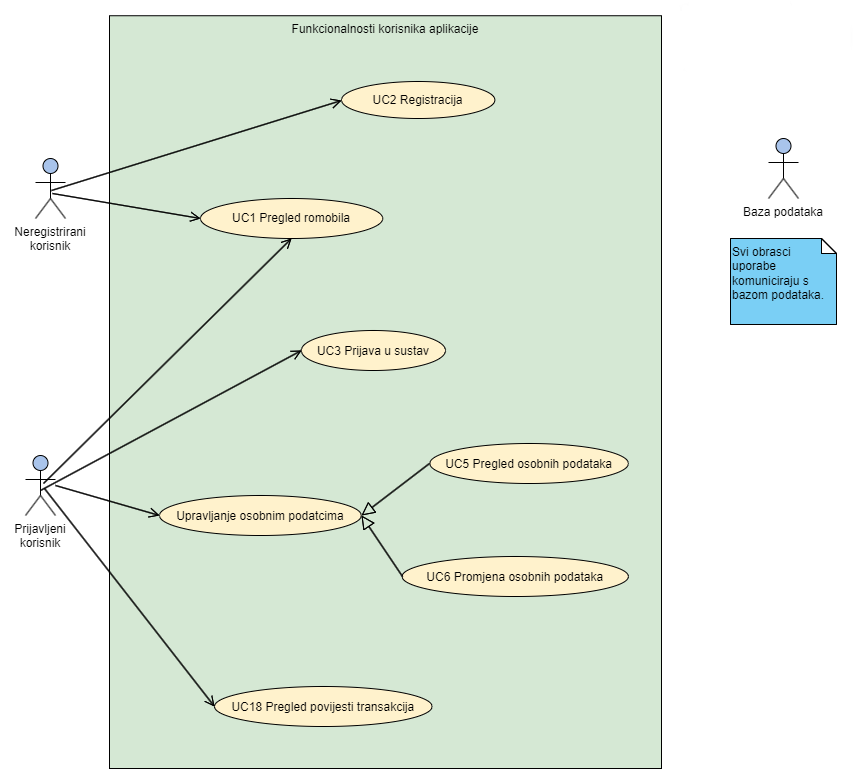
\includegraphics[width=0.8\textwidth]{dijagrami/korisnik.png}
						\caption{Dijagram obrasca uporabe, funkcionalnost korisnika}
						\label{fig:your_label}
					\end{figure}
					
					\begin{figure}[H]
						\centering
						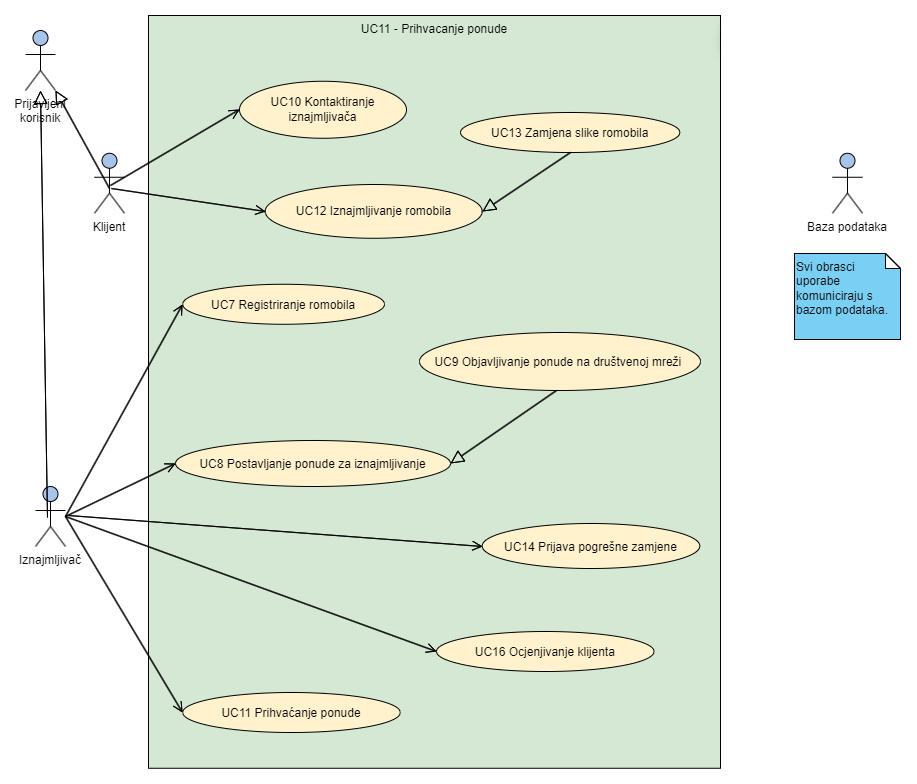
\includegraphics[width=0.8\textwidth]{dijagrami/klijent.png}
						\caption{Dijagram obrasca uporabe, funkcionalnost klijenta i iznajmljivača}
						\label{fig:your_label}
					\end{figure}
					
					\begin{figure}[H]
						\centering
						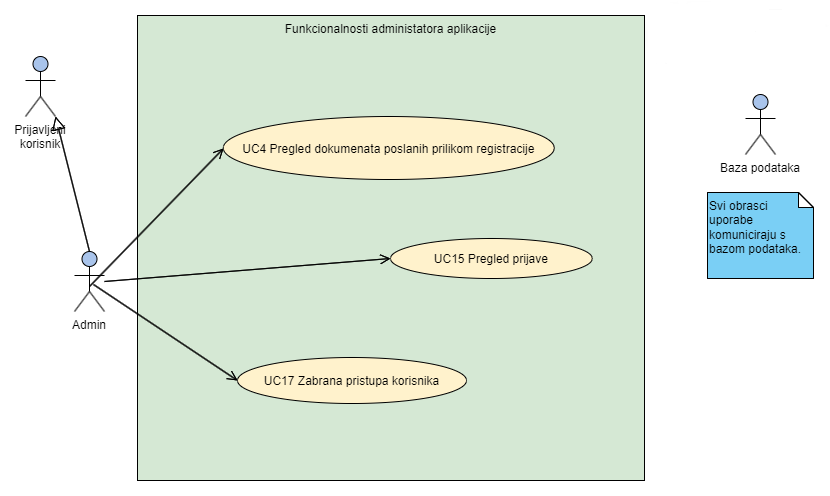
\includegraphics[width=0.8\textwidth]{dijagrami/admin.png}
						\caption{Dijagram obrasca uporabe, funkcionalnost administratora}
						\label{fig:your_label}
					\end{figure}

			\eject		
				
			\subsection{Sekvencijski dijagrami}
			
				\noindent \textbf{Obrazac uporabe UC15 – Pregled prijave}
				
				\noindent Administrator dobiva obavijest da je iznajmljivača podnio prijavu na zamjenu slika koju je izvršio klijent. Administrator pregledava izmijenjene slike i odlučuje hoće li se zamjena slika izvršiti ili ne. Administratorova odluka dolazi kao obavijest iznajmljivaču i korisniku. Ako je prijava potvrđena nema promjena u bazi, a u slučaju da nije, slike romobila se vraćaju na one prije izmjene.
				
				\begin{figure}[H]
					\centering
					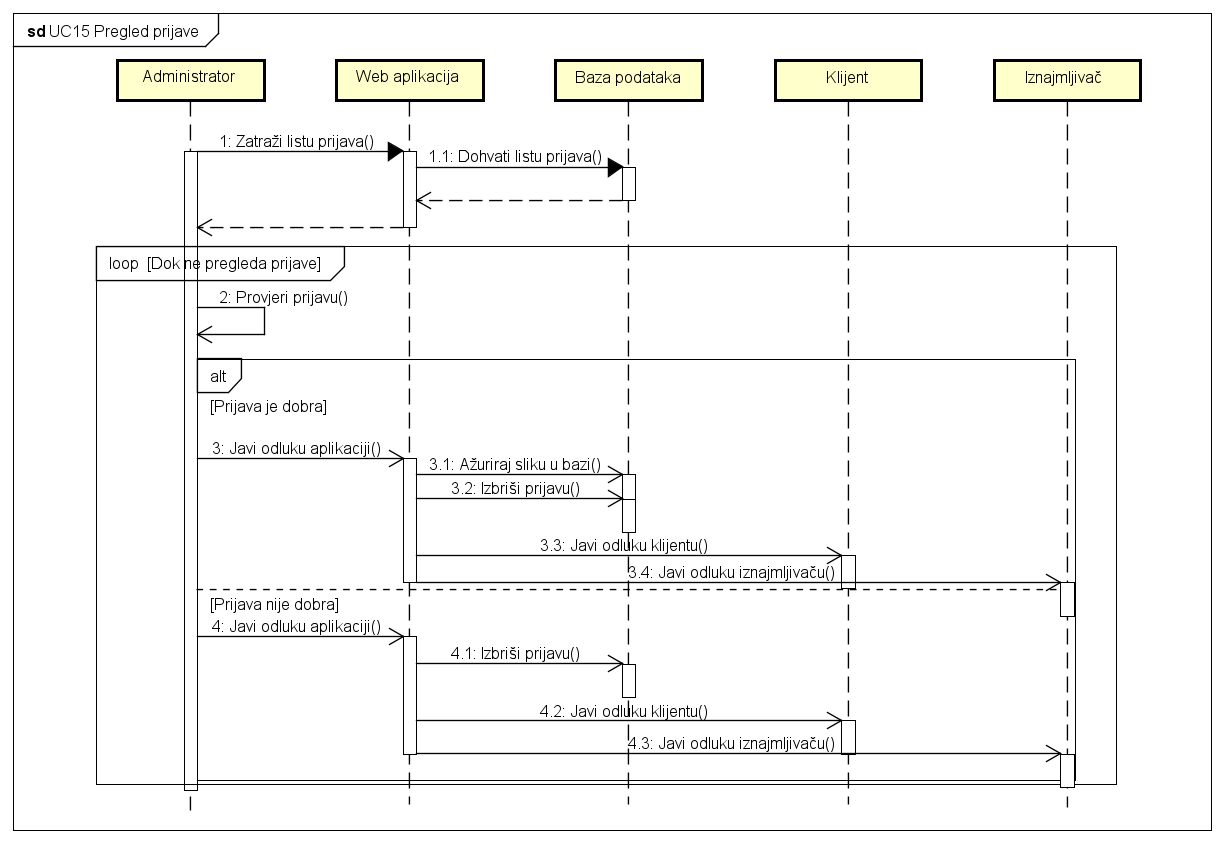
\includegraphics[width=0.8\textwidth]{dijagrami/UC15_Pregled_prijave.png}
					\caption{Sekvencijski dijagram za UC15}
					\label{fig:your_label}
				\end{figure}
				

				\eject


				\noindent \textbf{Obrazac uporabe UC12 – Iznajmljivanje romobila}
				
				\noindent Klijent inicira zahtjev za pregled dostupnih oglasa kako bi odabrao željeni romobil. Poslužitelj potom pristupa trenutnim oglasima iz baze podataka i prikazuje ih klijentu. Nakon odabira oglasa, poslužitelj povlači sve relevantne podatke o odabranom romobilu i predstavlja ih klijentu. Korisnik ima mogućnost provjeriti usklađenost prikazanih fotografija romobila s njegovim stvarnim stanjem. Kada klijent donese odluku, šalje zahtjev za iznajmljivanje romobila iznajmljivaču. Iznajmljivač ima opciju prihvatiti ili odbiti zahtjev klijenta. U slučaju prihvata, poslužitelj prosljeđuje relevantne podatke o rezervaciji romobila bazi podataka.

				
				\begin{figure}[H]
					\centering
					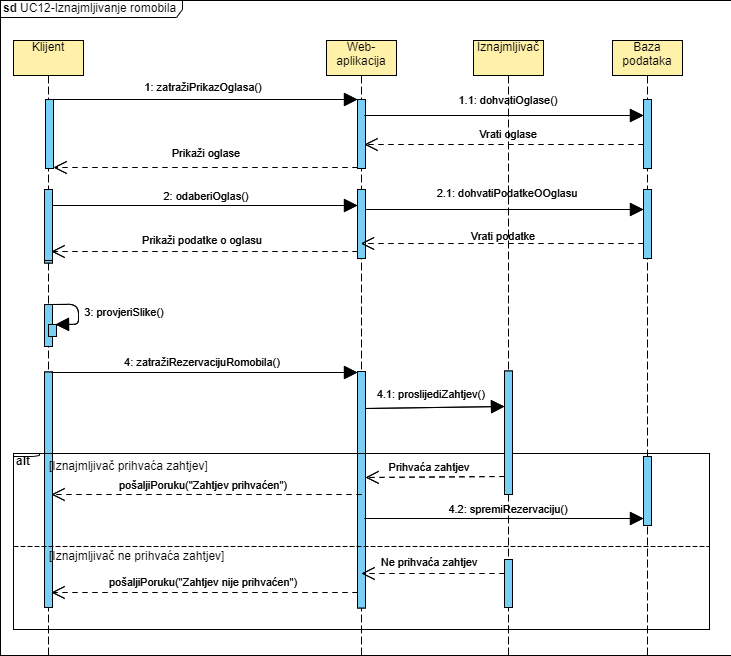
\includegraphics[width=0.8\textwidth]{dijagrami/sd_uc12.png}
					\caption{Sekvencijski dijagram za UC12}
					\label{fig:your_label}
				\end{figure}

				\eject
				
				\noindent \textbf{Obrazac uporabe UC16 – Ocjenjivanje klijenta}
				
				\noindent Iznajmljivač odabire klijenta kojemu onda on dodjeljuje ocjenu i komentar. Ukoliko nisu popunjena oba polja za ocjenu i komentar, aplikacija iznajmljivaču šalje poruku da nisu uneseni svi podaci te mo daje opciju ponovnog unosa. Tu poruku iznajmljivač dobiva za svaku takvu nepotpunu objavu. Iznajmljivač može tada odustati od objave ili nadopuniti. Ocjena i komentar su nakon toga vidljivi na profilu klijenata.

				
				\begin{figure}[H]
					\centering
					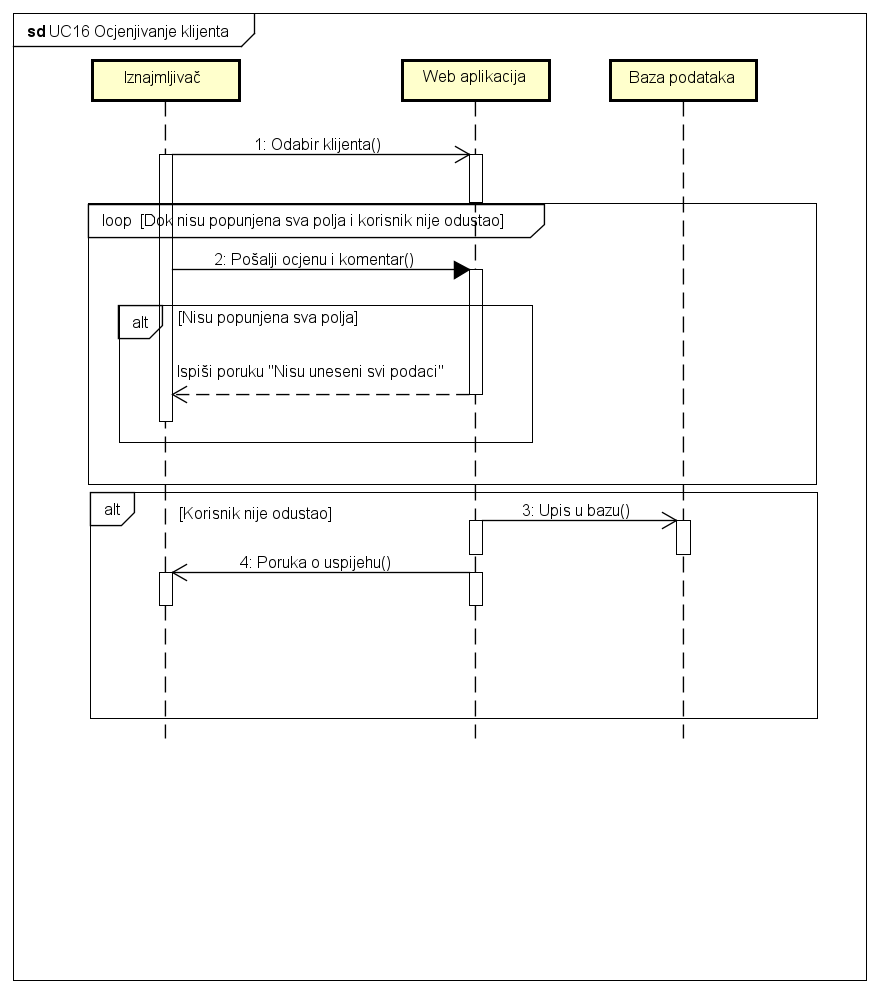
\includegraphics[width=0.8\textwidth]{dijagrami/UC16_Ocjenjivanje_klijenta.png}
					\caption{Sekvencijski dijagram za UC16}
					\label{fig:your_label}
				\end{figure}


				\eject


		\section{Ostali zahtjevi}
		
			\begin{packed_item} 
				\item Sustav treba omogućiti rad više korisnika u stvarnom vremenu
				\item Korisničko sučelje i sustav moraju podržavati hrvatsku abecedu (dijakritičke znakove) pri unosu i prikazu tekstualnog sadržaja
				\item Izvršavanje dijela programa u kojem se pristupa bazi podataka ne smije trajati duže od nekoliko sekundi 
				\item Sustav treba biti implementiran kao web aplikacija koristeći objektno-orijentirane jezike
				\item Neispravno korištenje korisničkog sučelja ne smije narušiti funkcionalnost i rad sustava
				\item
				Sustav treba biti jednostavan za korištenje, korisnici se moraju znati koristiti sučeljem bez opširnih uputa
				\item 
				Nadogradnja sustava ne smije narušavati postojeće funkcionalnosti sustava
				\item 
				Sustav kao valutu koristi EUR
				\item 
				Veza s bazom podataka mora biti kvalitetno zaštićena, brza i otporna na vanjske greške
				\item 
				Pristup sustavu mora biti omogućen iz javne mreže pomoću HTTPS.
			\end{packed_item}
			 
			 
			 
	
	\chapter{Arhitektura i dizajn sustava}
		
		\indent Odabrali smo arhitekturu klijent-poslužitelj zbog njezine skalabilnosti i jasne podjele odgovornosti između klijentskog i poslužiteljskog dijela sustava. Ova arhitektura pruža učinkovitu komunikaciju između korisničkog sučelja i servera. \\
		
		\indent Sustav je organiziran kao \textit{\underbar{klijent-poslužitelj}}, pri čemu klijent sadržava korisničko sučelje i logiku za interakciju s korisnikom. S druge strane, poslužitelj obrađuje zahtjeve klijenata, pristupa bazi podataka i upravlja poslovnim logikama. \\
		
		\indent \textit{\underbar{Aplikacija}} je strukturirana na slojevima, gdje frontend koristi React tehnologiju, koja obuhvaća korisničko sučelje i logiku za prikaz podataka korisnicima. Backend, s druge strane, koristi kombinaciju Java, JavaScript i Spring Boot tehnologija, obrađuje poslovnu logiku, upravlja pristupom bazi podataka i komunicira s klijentima. Ova struktura temelji se na \textit{\underbar{Model-View-Controller (MVC)}} arhitekturi, gdje model predstavlja podatke i poslovnu logiku, view je odgovoran za prikazivanje podataka, a controller upravlja korisničkim zahtjevima. \\
		
		\indent \textit{\underbar{Klijent}} radi na različitim uređajima, uključujući računala, pametne telefone i tablete, putem web preglednika. Poslužitelj je smješten u lokalnom data centru s potrebnim resursima za podršku poslužiteljskoj logici i bazi podataka. Baza podataka djeluje kao centralno spremište za pohranu podataka, s pristupom koji je kontroliran od strane poslužitelja. \\
		
		\indent Klijent inicira zahtjeve i prikazuje podatke korisnicima, dok poslužitelj obrađuje zahtjeve, upravlja poslovnim logikama te komunicira s bazom podataka. \\
		\indent Za komunikaciju između klijenta i poslužitelja koristimo HTTP/HTTPS, osiguravajući time sigurnu razmjenu podataka. Za pouzdan prijenos podataka između različitih komponenti sustava koristi se TCP/IP. \\
		
		\indent \textit{\underbar{Razvojna okolina}} uključuje korištenje Eclipse i Visual Studio Code za razvoj aplikacije, pružajući programerima učinkovite alate za pisanje, testiranje i održavanje koda tijekom razvojnog ciklusa. \\
				
		\section{Baza podataka}
			
			\noindent Za potrebe našeg sustava koristiti ćemo relacijsku bazu podataka koja svojom strukturom olakšava modeliranje stvarnog svijeta. Gradivna jedinka baze je relacija, odnosno tablica koja je definirana svojim imenom i skupom atributa. Zadaća baze podataka je brza i jednostavna pohrana, izmjena i dohvat podataka za daljnju obradu.
			Baza podataka ove aplikacije sastoji se od sljedećih entiteta:
			
			\begin{packed_item} 
				\item User
				\item Authority
				\item Scooter
				\item ScooterImages
				\item Listing
				\item Message
				\item ImageChangeRequest
				\item Rental
				\item Rating
				\item Transaction
			\end{packed_item}
				
		
			\subsection{Opis tablica}
			

				\textbf{User} entitet sadržava sve važne informacije o korisniku aplikacije. Sadrži atribute: email, nadimak, lozinku, ime, prezime, broj kartice za plaćanje, presliku osobne iskaznice te potvrdu o nekažnjavanju. Ovaj entitet u vezi je Many-to-One s entitetiom Authority, sa entitetom Scooter, Message te Rental.
				
				
				\begin{longtblr}[
					label=none,
					entry=none
					]{
						width = \textwidth,
						colspec={|X[10,l]|X[8, l]|X[20, l]|}, 
						rowhead = 1,
					} %definicija širine tablice, širine stupaca, poravnanje i broja redaka naslova tablice
					\hline \SetCell[c=3]{c}{\textbf{User}}	 \\ \hline[3pt]
					\SetCell{LightGreen}userID & INT	&  	Jedinstveni identifikator korisnika  	\\ \hline
					firstName	& VARCHAR &  Ime korisnika 	\\ \hline 
					lastName & VARCHAR &  Prezime korisnika  \\ \hline
					password & VARCHAR &  Hash lozinke  \\ \hline
					CardNumber & VARCHAR &   Broj kartice za plaćanje  \\ \hline
					email & VARCHAR &   Email adresa korisnika   \\ \hline
					idCard & MEDIUMTEXT &  Kopija osobne iskaznice  \\ \hline
					CertificateOfNo CriminalRecord & MEDIUMTEXT & Potvrda o nekažnjavanju korisnika  \\ \hline 
				\end{longtblr}
				
				\textbf{Authority} entitet pohranjuje informacije o ovlastima korisnika. Sadrži atribute: jedinstveni identifikator autorizacije, identifikator korisnika kojemu ovlast pripada i naziv ovlasti. U vezi je One-To-Many s entitetom User preko atributa jedinstvenog identifikatora korisnika.
				
				\begin{longtblr}[
					label=none,
					entry=none
					]{
						width = \textwidth,
						colspec={|X[10,l]|X[8, l]|X[20, l]|}, 
						rowhead = 1,
					} %definicija širine tablice, širine stupaca, poravnanje i broja redaka naslova tablice
					\hline \SetCell[c=3]{c}{\textbf{Authority}}	 \\ \hline[3pt]
					\SetCell{LightGreen}authorityID & INT	&  	Jedinstveni identifikator autorizacije 	\\ \hline
					\SetCell{LightBlue}userID & INT	&  	Jedinstveni identifikator korisnika  \\ \hline 
					authority	& VARCHAR &  Naziv ovlasti 	\\ \hline 
				\end{longtblr}
				
				\textbf{Scooter} entitet pohranjuje informacije o romobilu koji se iznajmljuje. Sadrži atribute: jedinstveni identifikator romobila te jedinstveni identifikator vlasnika. U vezi je One-to-Many sa entitom User preko njegovog identifikatora te Many-To-One sa entitetom ScooterImages.
				
				\begin{longtblr}[
					label=none,
					entry=none
					]{
						width = \textwidth,
						colspec={|X[10,l]|X[8, l]|X[20, l]|}, 
						rowhead = 1,
					} %definicija širine tablice, širine stupaca, poravnanje i broja redaka naslova tablice
					\hline \SetCell[c=3]{c}{\textbf{Scooter}}	 \\ \hline[3pt]
					\SetCell{LightGreen}scooterID & INT	&  	Jedinstveni identifikator romobila 	\\ \hline
					\SetCell{LightBlue}ownerID & INT	&  	Jedinstveni identifikator vlasnika romobila  \\ \hline 
				\end{longtblr}
				
				\textbf{Listing} entitet pohranjuje informacije o oglasu za iznajmljivanje romobila. Sadrži atribute: jedinstveni identifikator oglasa, jedinstveni identifikator romobila, lokaciju romobila, lokaciju povratka romobila, krajnje vrijeme povratka romobila, cijenu najma po prijeđenom kilometru, iznos novčane kazne u slučaju ne vraćanja romobila na vrijeme te status oglasa. U vezi je Many-To-One s entitetom Scooter preko identifikatora romobila.
				
				\begin{longtblr}[
					label=none,
					entry=none
					]{
						width = \textwidth,
						colspec={|X[10,l]|X[8, l]|X[20, l]|}, 
						rowhead = 1,
					} %definicija širine tablice, širine stupaca, poravnanje i broja redaka naslova tablice
					\hline \SetCell[c=3]{c}{\textbf{Listing}}	 \\ \hline[3pt]
					\SetCell{LightGreen}listingID & INT	&  	Jedinstveni identifikator oglasa	\\ \hline
					\SetCell{LightBlue}scooterID & INT	&  	Jedinstveni identifikator romobila  \\ \hline 
					location & VARCHAR &  Lokacija romobila	\\ \hline 
					returnLocation & VARCHAR &  Lokacija za povratak romobila	\\ \hline 
					returnByTime & DATETIME &  Vrijeme do kada romobil mora biti vraćen  \\ \hline
					pricePerKilometer & VARCHAR & Cijena iznajmljivanja po kilometru  \\ \hline
					lateReturnPenalty & VARCHAR & Iznos zakasnine kod vraćanja romobila  \\ \hline
					status & VARCHAR & Status oglasa (aktivno, završeno) \\ \hline
				\end{longtblr}
				
				\textbf{Message} entitet sadržava sve važne informacije o porukama između iznajmljivača i unajmitelja. Sadrži atribute: jedinstveni identifikator poruka, identifikator pošiljatelja i primatelja poruke, vrijeme slanja poruke, tekst poruke i jedinstveni identifikator oglasa na kojeg se korisnik javlja. Ovaj entitet u vezi je Many-to-One s User preko jedinstvenog identifikatora pošiljatelja, u vezi Many-to-One s User preko jedinstvenog identifikatora primatelja i u vezi Many-to-One s Listing preko jedinstvenog identifikatora oglasa.
				
				\begin{longtblr}[
					label=none,
					entry=none
					]{
						width = \textwidth,
						colspec={|X[10,l]|X[8, l]|X[20, l]|}, 
						rowhead = 1,
					} %definicija širine tablice, širine stupaca, poravnanje i broja redaka naslova tablice
					\hline \SetCell[c=3]{c}{\textbf{Message}}	 \\ \hline[3pt]
					\SetCell{LightGreen}messageID & INT	&  	Jedinstveni identifikator poruke\\ \hline
					\SetCell{LightBlue}userFromID & INT	&  	Jedinstveni identifikator pošiljatelja  \\ \hline
					\SetCell{LightBlue}userToID & INT	&  	Jedinstveni identifikator primatelja  \\ \hline 
					\SetCell{LightBlue}listingID & INT	&  	Jedinstveni identifikator oglasa  \\ \hline
					content & VARCHAR & Sadržaj poruke  \\ \hline
					sentAt & DATETIME & vrijeme slanja poruke  \\ \hline
				\end{longtblr}
				
				\textbf{ImageChangeRequest} entitet pohranjuje zahtjeve korisnika za promjenu slike romobila kojeg su unajmili. Sadrži atribute: jedinstveni identifikator najma romobila, novu sliku romobila, identifikator trenutne fotografije koju želimo zamijeniti te razlog zamjene priloženu uz zahtjev. U vezi je One-To-One sa ScooterImages te Many-To-One sa Rental entitetom.
				
				\begin{longtblr}[
					label=none,
					entry=none
					]{
						width = \textwidth,
						colspec={|X[10,l]|X[8, l]|X[20, l]|}, 
						rowhead = 1,
					} %definicija širine tablice, širine stupaca, poravnanje i broja redaka naslova tablice
					\hline \SetCell[c=3]{c}{\textbf{ImageChangeRequest}}	 \\ \hline[3pt]
					\SetCell{LightGreen}imageChange RequestID & INT	&  	Jedinstveni identifikator zahtjeva za promjenu slike romobila	\\ \hline
					replacementImage & MEDIUMTEXT & Slika stanja romobila kojom želimo zamijeniti postojeću  \\ \hline
					message & VARCHAR & Razlog zamijene slike romobila  \\ \hline
					\SetCell{LightBlue}rentalID & INT	&  	Jedinstveni identifikator najma romobila \\ \hline
					\SetCell{LightBlue}imageID & INT	&  	Jedinstveni identifikator fotografije romobila  \\ \hline
				\end{longtblr}
				
				\textbf{Rental} entitet sadržava sve važne informacije o najmu romobila. Sadrži atribute: jedinstveni identifikator najma romobila, jedinstveni identifikator unajmitelja, jedinstveni identifikator oglasa, početno vrijeme najma romobila i završno vrijeme najma romobila. Ovaj entitet u vezi je Many-to-One s entitetom User preko identifikatora unajmitelja, također Many-to-One s entitetom Listing. U vezi One-to-One s entitetom Transaction te u vezi One-to-One s entitetom Rating preko atributa jedinstveni identifikator najma romobila.
				
				\begin{longtblr}[
					label=none,
					entry=none
					]{
						width = \textwidth,
						colspec={|X[10,l]|X[8, l]|X[20, l]|}, 
						rowhead = 1,
					} %definicija širine tablice, širine stupaca, poravnanje i broja redaka naslova tablice
					\hline \SetCell[c=3]{c}{\textbf{Rental}}	 \\ \hline[3pt]
					\SetCell{LightGreen}rentalID & INT	&  	Jedinstveni identifikator najma romobila	\\ \hline
					\SetCell{LightBlue}renterID & INT	&  	Jedinstveni identifikator unajmitelja  \\ \hline
					\SetCell{LightBlue}listingID & INT	&  	Jedinstveni identifikator oglasa  \\ \hline
					rentalTimeStart & DATETIME & Početno vrijeme najma romobila  \\ \hline
					rentalTimeEnd & DATETIME & Završno vrijeme najma romobila  \\ \hline
				\end{longtblr}
				
				\textbf{Rating} entitet sadrži sve bitne informacije o ocjenjivanju korisnika. Sadrži atribute: jedinstveni identifikator ocjene, identifikator najma romobila, ocjenu korisnika, komentar te vrijeme postavljanja ocjene. U vezi je One-To-One sa entitetom Rental preko identifikatora najma romobila.
				
				\begin{longtblr}[
					label=none,
					entry=none
					]{
						width = \textwidth,
						colspec={|X[10,l]|X[8, l]|X[20, l]|}, 
						rowhead = 1,
					} %definicija širine tablice, širine stupaca, poravnanje i broja redaka naslova tablice
					\hline \SetCell[c=3]{c}{\textbf{Rating}}	 \\ \hline[3pt]
					\SetCell{LightGreen}ratingID & INT	&  	Jedinstveni identifikator ocjene	\\ \hline
					\SetCell{LightBlue}rentalID & INT	&  	Jedinstveni identifikator najma romobila	\\ \hline
					grade & VARCHAR & Ocjena korisnika  \\ \hline
					comment & VARCHAR & Komentar  \\ \hline
					ratingTime & DATETIME & Vrijeme ocjenjivanja korisnika \\ \hline
				\end{longtblr}
				
				\textbf{Transaction} Ovaj entitet pohranjuje informacije o jednoj transakciji. Sadrži atribute: identifikator transakcije, identifikator najma, broj prijeđenih kilometara te ukupnu cijenu najma. U vezi je One-To-One s entitetom Rental.
				
				\begin{longtblr}[
					label=none,
					entry=none
					]{
						width = \textwidth,
						colspec={|X[10,l]|X[8, l]|X[20, l]|}, 
						rowhead = 1,
					} %definicija širine tablice, širine stupaca, poravnanje i broja redaka naslova tablice
					\hline \SetCell[c=3]{c}{\textbf{Transaction}}	 \\ \hline[3pt]
					\SetCell{LightGreen}transactionID & INT	&  	Jedinstveni identifikator transakcije	\\ \hline
					\SetCell{LightBlue}rentalID & INT	&  	Jedinstveni identifikator najma romobila	\\ \hline
					totalPrice & VARCHAR & Ukupna cijena najma romobila  \\ \hline
					kilometersPassed & VARCHAR & Kilometri prijeđeni romobilom  \\ \hline
					timeOfTransaction & DATETIME &  Vrijeme transakcije  \\ \hline
				\end{longtblr}
				
				\textbf{ScooterImages} entitet sadrži fotografije vezane za romobil koji se iznajmljuje. Sadrži atribute: identifikator fotografije, identifikator romobila te samu sliku romobila. U vezi je Many-To-One sa entitetom Scooter preko identifikatora romobila.
				
				\begin{longtblr}[
					label=none,
					entry=none
					]{
						width = \textwidth,
						colspec={|X[10,l]|X[8, l]|X[20, l]|}, 
						rowhead = 1,
					} %definicija širine tablice, širine stupaca, poravnanje i broja redaka naslova tablice
					\hline \SetCell[c=3]{c}{\textbf{ScooterImages}}	 \\ \hline[3pt]
					\SetCell{LightGreen}imageID & INT	&  	Jedinstveni identifikator fotgrafije romobila	\\ \hline
					\SetCell{LightBlue}scooterID & INT	&  	Jedinstveni identifikator romobila  \\ \hline
					image & MEDIUMTEXT & Fotografija romobila  \\ \hline
				\end{longtblr}
				
			
			\subsection{Dijagram baze podataka}
			
				\begin{figure}[H]
					\centering
					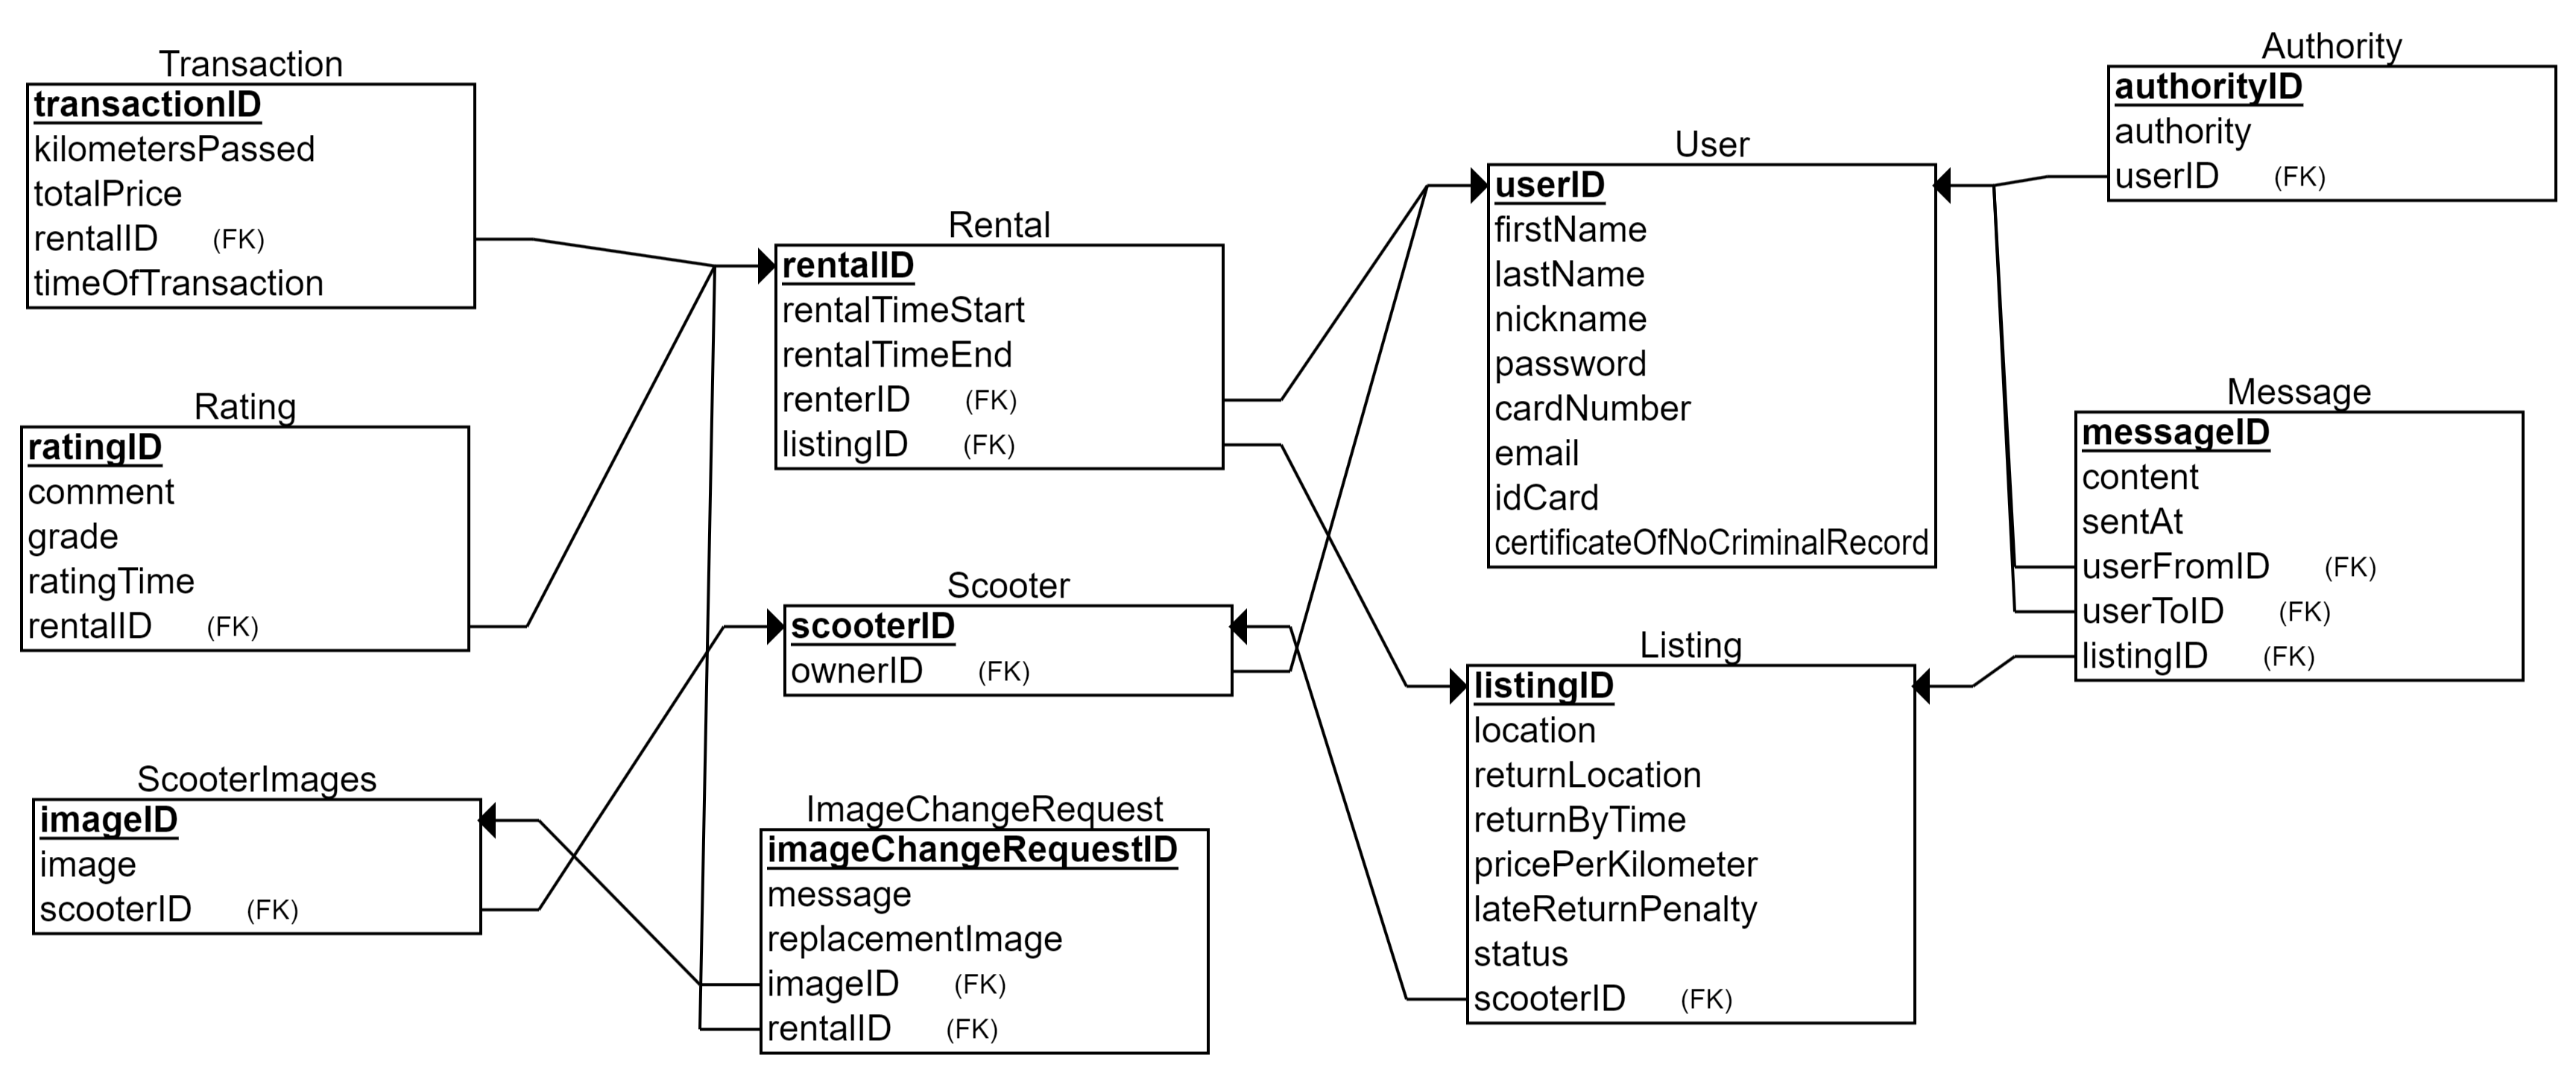
\includegraphics[width=0.8\textwidth]{dijagrami/relacijski_model_baza.png}
					\caption{E-R dijagram baze podataka}
					\label{fig:your_label}
				\end{figure}
			
			\eject
			
			
		\section{Dijagram razreda}
		
			\noindent Dijagrami razreda predstavljaju skup razreda koji su dio backend segmenta MVC arhitekture. Ti razredi nasljeđuju Controller razred. Metode unutar tih razreda manipuliraju s DTO (Data Transfer Object) koji su dohvaćeni kroz implementirane metode u Entitet i Servisi razredima. Kontrolni razredi implementiraju metode koje vraćaju JSON datoteke s odgovarajućim HTML status kodom. \\
			
			\indent Razredi su logički grupirani prema pravima pristupa određenih aktera. Ova organizacija pomaže smanjiti prenapučenost unutar dijagrama, gdje su prikazane samo ovisnosti između razreda koji pripadaju istom segmentu dijagrama. Informacije o nazivima i tipovima atributa unutar razreda omogućuju zaključivanje vrste ovisnosti među različitim razredima. \\
		
			\begin{figure}[H]
				\centering
				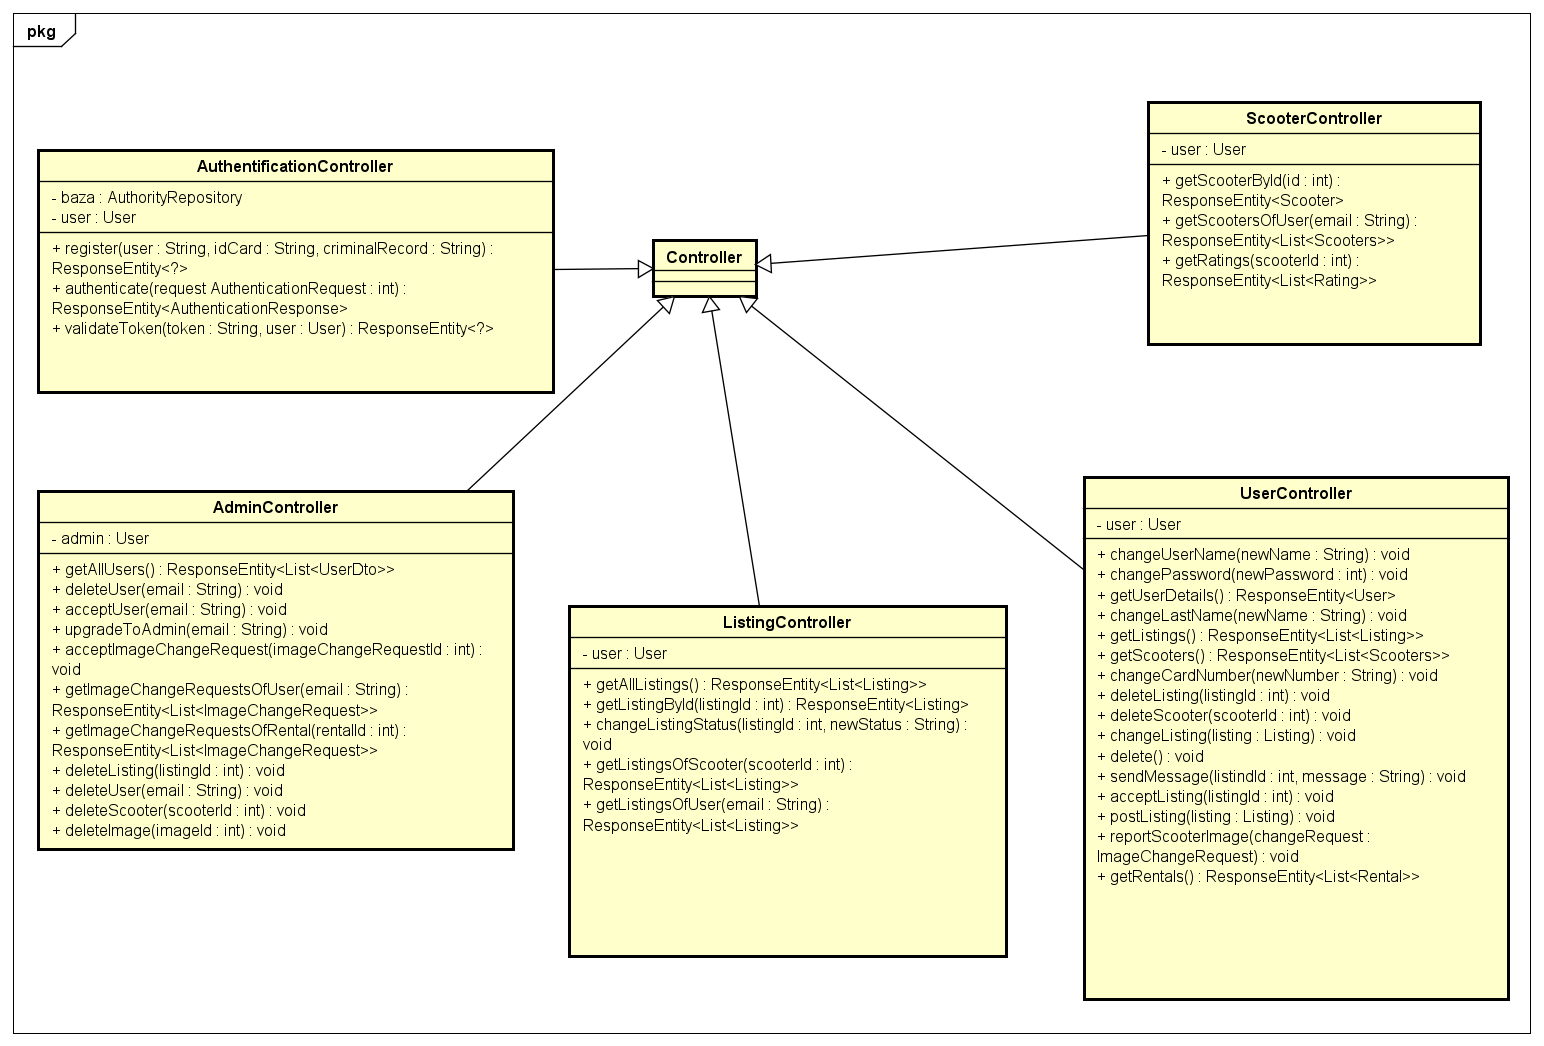
\includegraphics[width=0.8\textwidth]{dijagrami/ControllersDiagram.png}
				\caption{Dijagram razreda - dio Controllers}
				\label{fig:your_label}
			\end{figure}
			
			\begin{figure}[H]
				\centering
				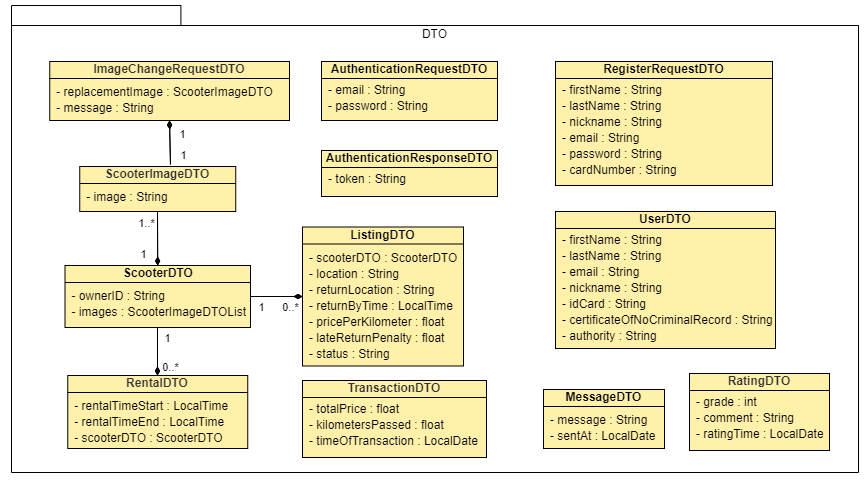
\includegraphics[width=0.8\textwidth]{dijagrami/DTO_dijagram.png}
				\caption{Dijagram razreda - dio Data Transfer Objects}
				\label{fig:your_label}
			\end{figure}
			
			\indent Servisi i Entiteti predstavljaju dvije ključne komponente koji primjenjuju arhitektonski obrazac poznat kao "Service-Oriented Architecture" (SOA) ili "Domain-Driven Design" (DDD). \\
			
			 \indent Entiteti predstavljaju objekte u bazi podataka koji imaju svoj identitet. Svaki entitet ima svoje primarne i sekundarne ključeve kojima su vezani za ostale entitete. \\
			 
			 \indent Servisi predstavljaju komponente sustava koje obavljaju određene operacije ili funkcionalnosti. Oni sadrže poslovnu logiku i nude specifične usluge koje se mogu pozvati iz drugih dijelova sustava. \\
			 
			\begin{figure}[H]
				\centering
				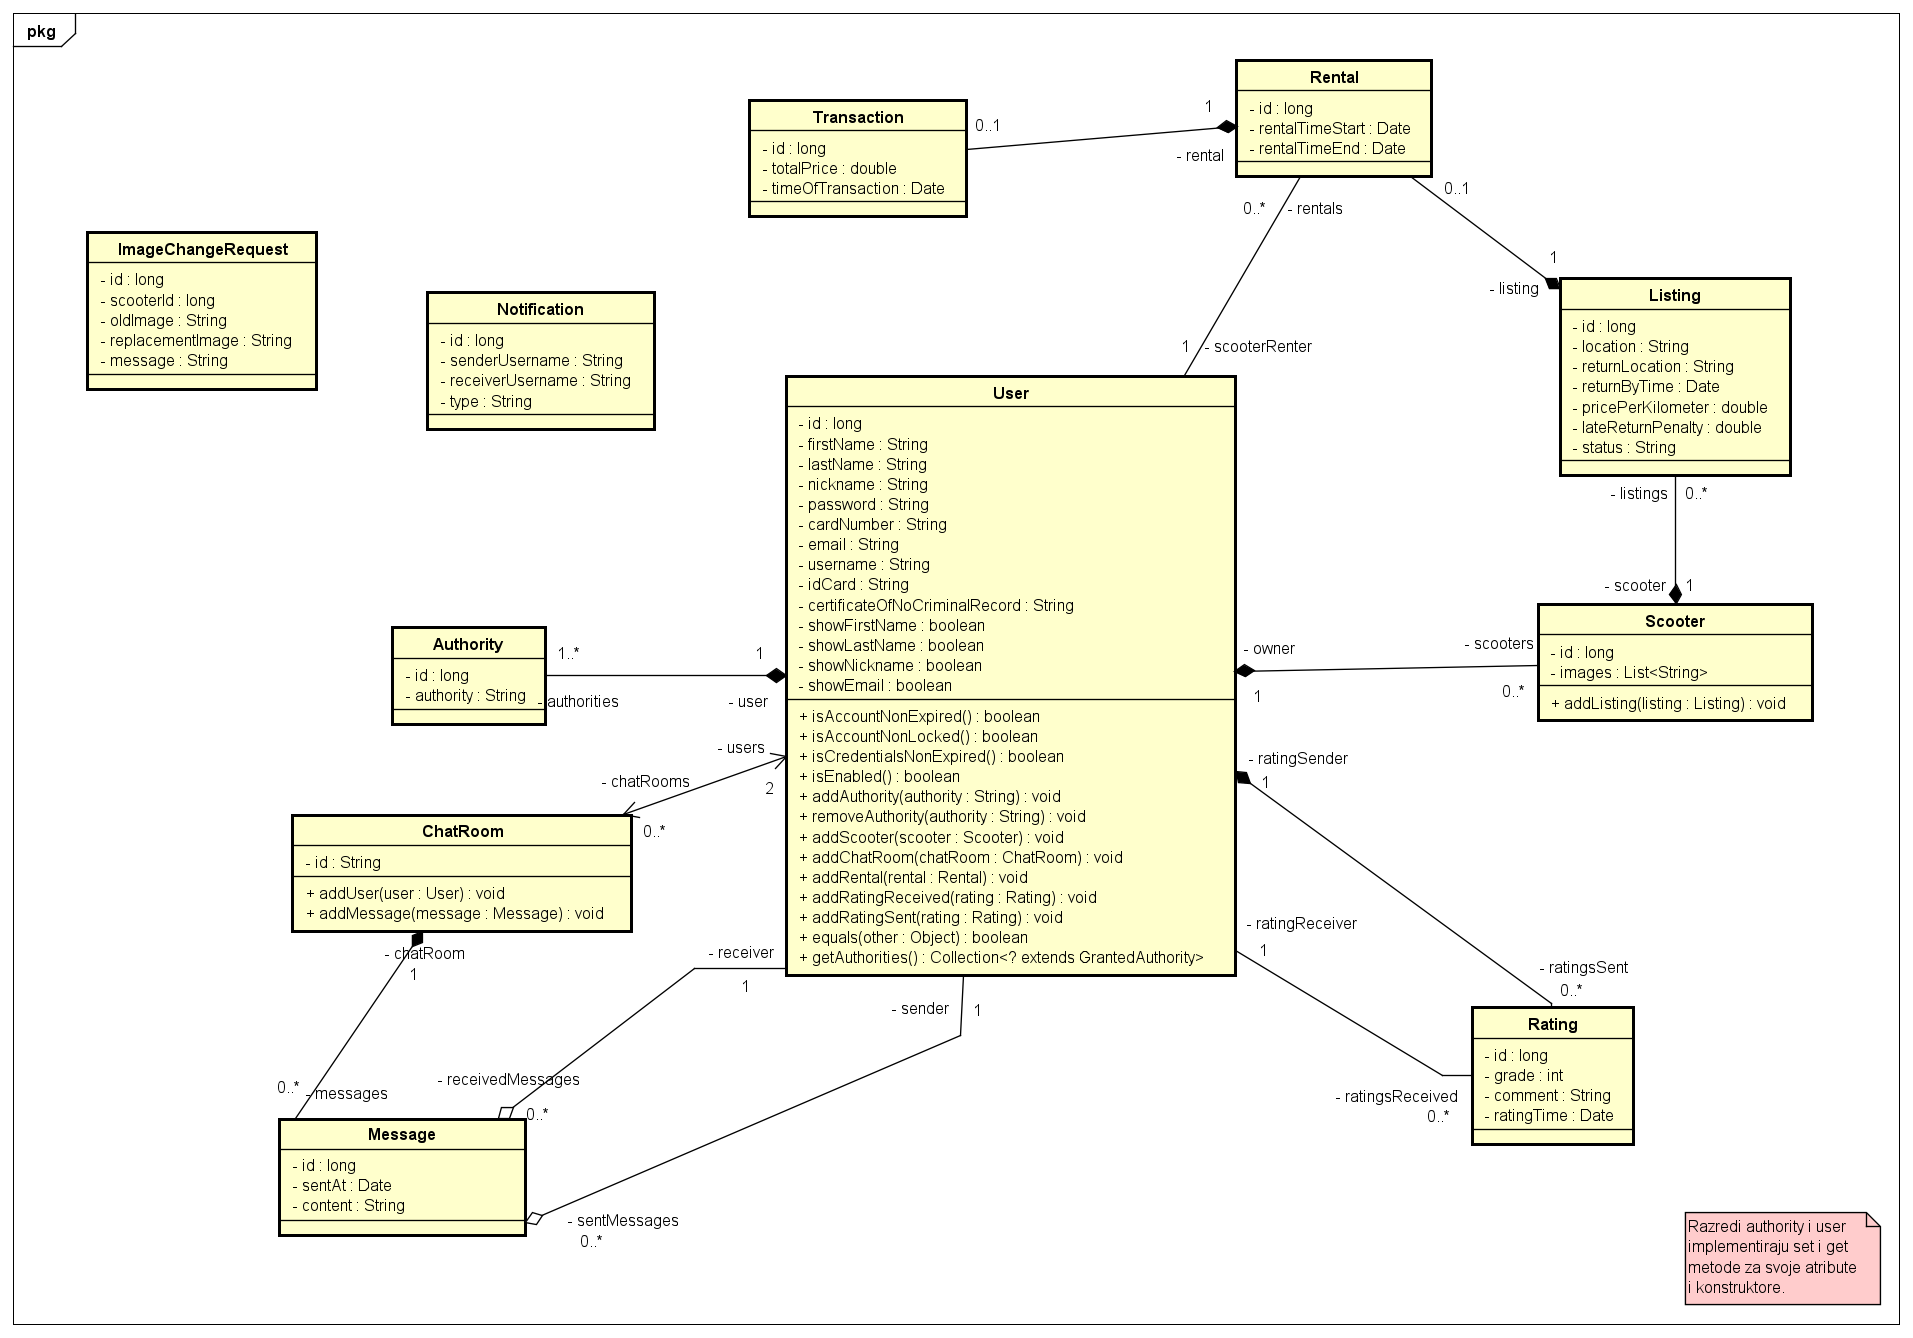
\includegraphics[width=0.8\textwidth]{dijagrami/entiteti.png}
				\caption{Dijagram razreda - dio Entiteti}
				\label{fig:your_label}
			\end{figure}
			
			\begin{figure}[H]
				\centering
				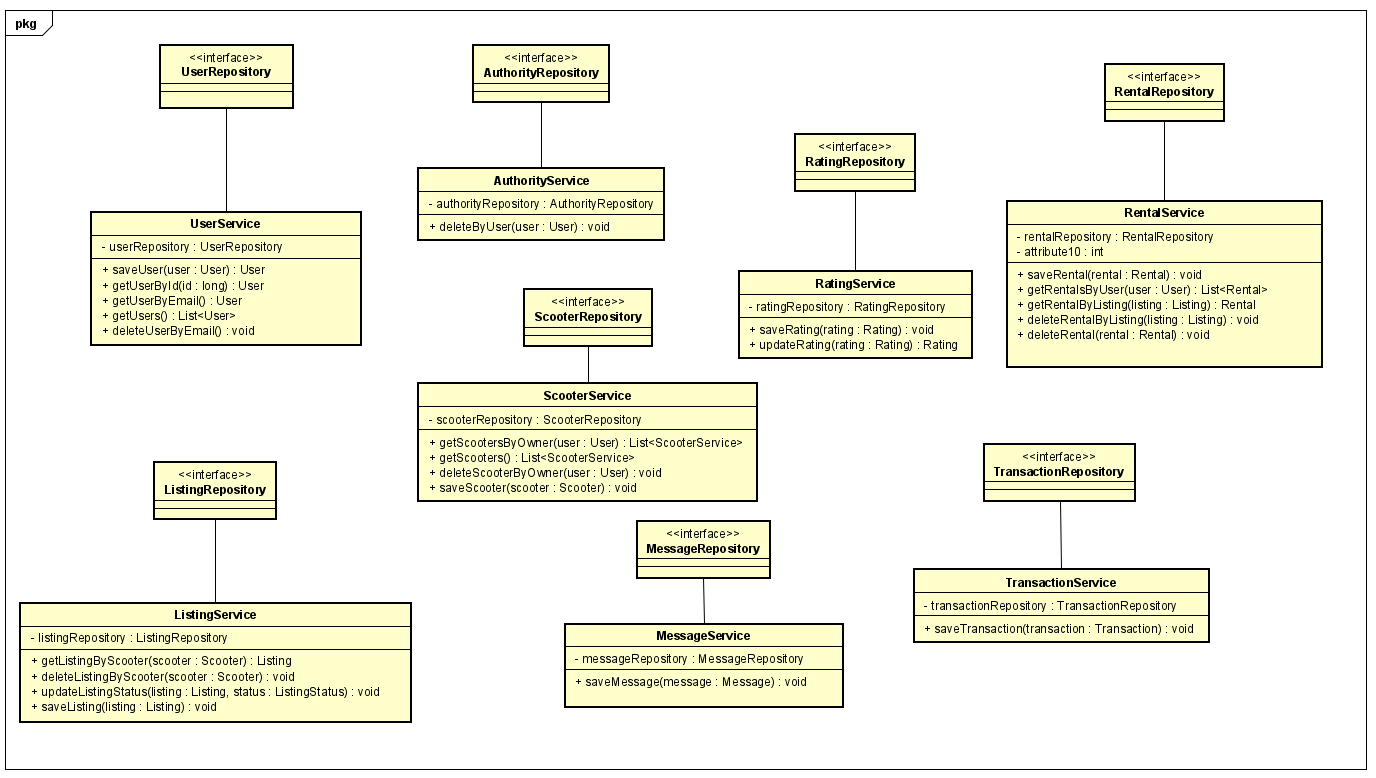
\includegraphics[width=0.8\textwidth]{dijagrami/servisi.png}
				\caption{Dijagram razreda - dio Servisi}
				\label{fig:your_label}
			\end{figure}
			
			
			\eject
		
		\section{Dijagram stanja}
			
			
			\textbf{\textit{dio 2. revizije}}\\
			
			\textit{Potrebno je priložiti dijagram stanja i opisati ga. Dovoljan je jedan dijagram stanja koji prikazuje \textbf{značajan dio funkcionalnosti} sustava. Na primjer, stanja korisničkog sučelja i tijek korištenja neke ključne funkcionalnosti jesu značajan dio sustava, a registracija i prijava nisu. }
			
			
			\eject 
		
		\section{Dijagram aktivnosti}
			
			\textbf{\textit{dio 2. revizije}}\\
			
			 \textit{Potrebno je priložiti dijagram aktivnosti s pripadajućim opisom. Dijagram aktivnosti treba prikazivati značajan dio sustava.}
			
			\eject
		\section{Dijagram komponenti}
		
			\textbf{\textit{dio 2. revizije}}\\
		
			 \textit{Potrebno je priložiti dijagram komponenti s pripadajućim opisom. Dijagram komponenti treba prikazivati strukturu cijele aplikacije.}
	\chapter{Implementacija i korisničko sučelje}
		
		
		\section{Korištene tehnologije i alati}
		
			Komunikacija u timu odvijala se videopozivima putem aplikacije \underline{\href{https://www.microsoft.com/en-us/microsoft-teams/group-chat-software}{Microsoft Teams}}\textsuperscript{1}. Za izradu UML dijagrama korišteni su alati \underline{\href{https://astah.net/products/astah-uml/}{Astah UML}}\textsuperscript{2} i \underline{\href{https://online.visual-paradigm.com/}{Visual Paradigm}}\textsuperscript{3}. \underline{\href{https://git-scm.com/}{Git}}\textsuperscript{4} je korišten kao sustav za upravljanje kodom. Projekt je dostupan na web platformi \underline{\href{https://github.com/}{GitHub}}\textsuperscript{5}
			
			\indent Za razvoj aplikacije korištena su razvojna okruženja \underline{\href{https://www.jetbrains.com/idea/}{IntelliJ IDE}}\textsuperscript{6} i \newline\underline{\href{https://code.visualstudio.com/}{Visual Studio Code}}\textsuperscript{7}. IntelliJ jedano je od najpopularnijih razvojnih okruženja za razvoj aplikacija u programskom jeziku Java. Izgradila ga je tvrtka JetBrains. Pruža bogatu podršku za razvoj desktop i web aplikacija. Visual Studio Code je također vrlo popularan uređivač za pisanje programskog koda, osobita za razvoj frontend dijela aplikacija jer pruža izrazito dobru podršku za frotend radne okvire. On je pod vlasištvom tvrtke Microsoft.
			
			\indent Aplikacija je napisana koristeći radni okvir \underline{\href{https://spring.io/projects/spring-boot/}{Spring Boot}}\textsuperscript{8} i jezik \underline{\href{https://www.oracle.com/java/}{Java}}\textsuperscript{9} za izradu \textit{backenda} te \underline{\href{https://react.dev/}{React}}\textsuperscript{10} i jezik \underline{\href{https://www.javascript.com/}{JavaScript}}\textsuperscript{11} za izradu \textit{frontenda}. React je bilioteka izražena u JavaScriptu koja olakšava izradu korisničkog sučelja. React je održava tvrtka Meta. Radni okvir Spring Boot nadograđuje mogućnosti samog programskog jezika Java te time uvelike olakšava razvoj web aplikacija. Nudi niz gotovih funkcionalnosti koji povećavaju produktivnost i efikasnost programera.
			
			\indent Za bazu podataka korišten je \underline{\href{https://www.postgresql.org/}{PostgreSQL}}\textsuperscript{12}.
			\noindent\\[1ex]\rule{0.5\linewidth}{0.5pt}\newline
			\noindent\textsuperscript{1}\url{https://www.microsoft.com/en-us/microsoft-teams/group-chat-software}\newline
			\noindent\textsuperscript{2}\url{https://astah.net/products/astah-uml/}\newline
			\noindent\textsuperscript{3}\url{https://online.visual-paradigm.com/}\newline
			\noindent\textsuperscript{4}\url{https://git-scm.com/}\newline
			\noindent\textsuperscript{5}\url{https://github.com/}\newline
			\noindent\textsuperscript{6}\url{https://www.jetbrains.com/idea/}\newline
			\noindent\textsuperscript{7}\url{https://code.visualstudio.com/}\newline
			\noindent\textsuperscript{8}\url{https://spring.io/projects/spring-boot/}\newline
			\noindent\textsuperscript{9}\url{https://www.oracle.com/java/}\newline
			\noindent\textsuperscript{10}\url{https://react.dev/}\newline
			\noindent\textsuperscript{11}\url{https://www.javascript.com/}\newline
			\noindent\textsuperscript{12}\url{https://www.postgresql.org/}\newline
			
		\newpage
		
		\section{Ispitivanje programskog rješenja}
			
			\indent Za provođenje testiranja naše Spring Boot aplikacije koristili smo biblioteke JUnit i Mockito. One su nam omogućile pouzdano i sustavno testiranje raličitih dijelova aplikacije. Za ispitivanje sustava koristili smo alat Selenium.
			 
	
			
			\subsection{Ispitivanje komponenti}
			U nastavku ovog poglavlja, pronaći ćete detaljan opis šest odabranih ispitnih slučajeva koji obuhvaćaju redovne situacije, rubne uvjete te testiranje ponašanja sustava u situacijama iznimki. Uz opis ispitnih slučajeva, priložili smo i odgovarajući izvorni kôd svakog testa, kao i rezultate izvođenja ispita u razvojnom okruženju, što omogućuje transparentnost i preglednost provedenih ispitivanja.
			
			Prvi test koji smo odradili je dohvaćanje romobila preko njegovog identifikatora. U ovom smo testu testirali servisni sloj naše aplikacije te set test uredno proveo.
			\begin{figure}[h]
				\centering
				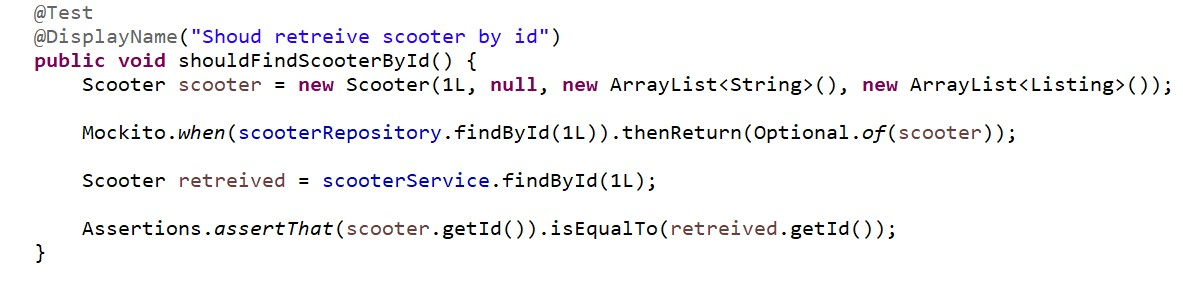
\includegraphics[width=0.6\textwidth]{slike/scooter_service_test.jpg}
				\caption{Testiranje dohvaćanja romobila preko identifikatora}
				\label{fig:Testiranje dohvaćanja romobila preko identifikatora}
			\end{figure}
			
			U sljedećem testu također smo testirali servisni sloj i to dohvaćanje poruka za dva korisnika. Dakle, u testu definiramo dva korisnika te provjeravamo vraća li nam naša aplikacija tražene poruke.
			\begin{figure}[h]
				\centering
				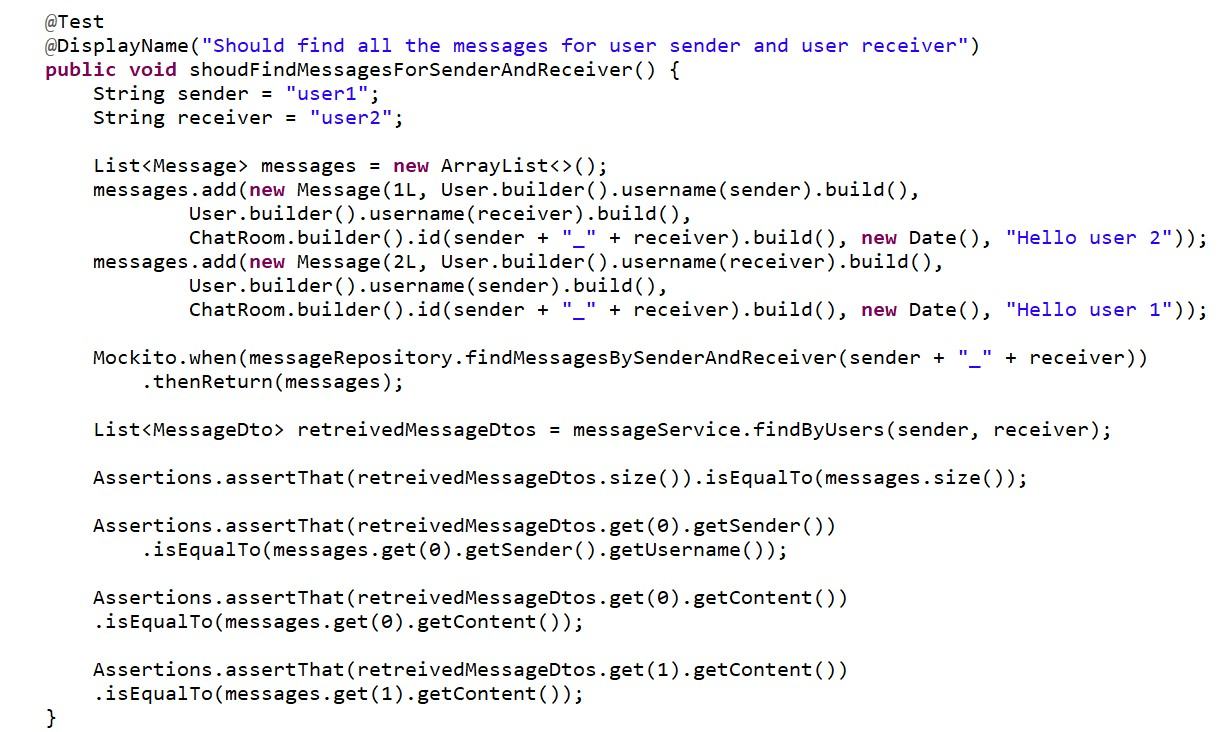
\includegraphics[width=0.6\textwidth]{slike/message_service_test.jpg}
				\caption{Testiranje dohvaćanja poruka za zadene korisnike}
				\label{fig:Testiranje dohvaćanja poruka za zadene korisnike}
			\end{figure}
			
			Sada ćemo prikazati testiranje ListingController. U prvom testu testirali smo dodavanje novog oglasa te je očekivani ishod odgovor poslužitelja sa novim oglasom, dok smo u drugom pokušali dohvatit oglas za nepostojeći romobil. U drugom testu očekuujemo da poslužitelj baci novu NullPointerException iznimku. Oba testa su se izvršila ispravno. \newline
			
			  \begin{figure}
					  	\centering
					  	\subfigure{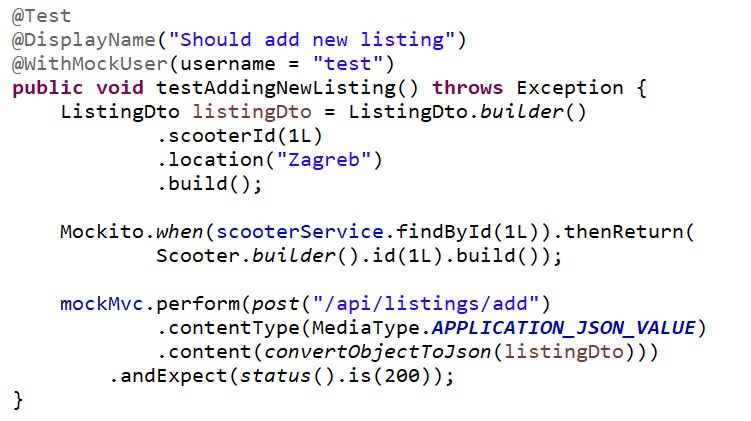
\includegraphics[width=0.4\textwidth]{slike/listing_controller_add_test.jpg}} 
					  	\subfigure{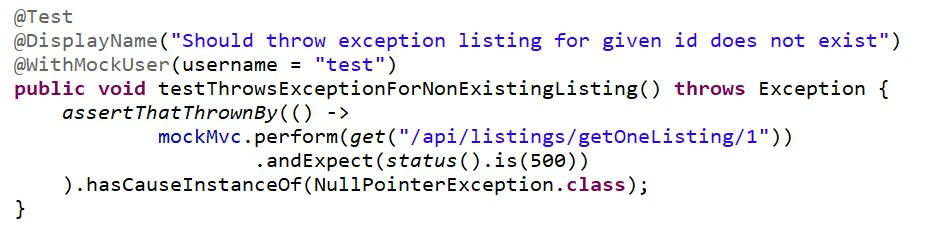
\includegraphics[width=0.4\textwidth]{slike/listing_controller_throw_test.jpg}} 
					  	\caption{Testiranje ListingController-a}
					  	\label{fig:Testiranje ListingController-a}
			  \end{figure}
			  
			Korisnik mora moći pregledavati romobile koje je trenutno iznajmio pa smo testirali i RentalController i to metodu koja osigurava dohvaćanje trenutnih najmova. U testu definiramo koje objekte tipa Rental očekujemo te kada primimo odgovor od poslužitelja provjeravamo jesmo li ih uistinu i primili. \newline
			
			\begin{figure}[h]
				\centering
				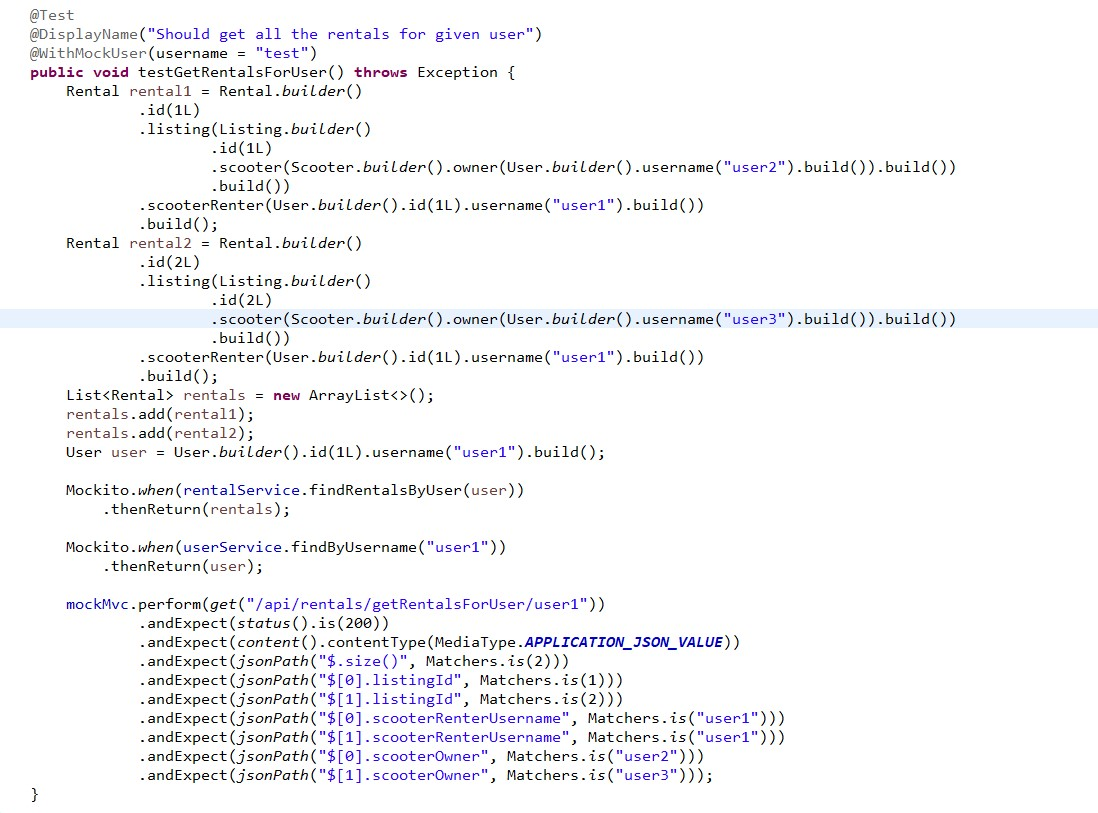
\includegraphics[width=0.6\textwidth]{slike/rental_controller_test.jpg}
				\caption{Testiranje dohvaćanja najmova za korisnika}
				\label{fig:Testiranje dohvaćanja najmova za korisnika}
			\end{figure}
			
			Na kraju, provjerili smo što će se dogodit ako pokušamo izbrisat ocjenu i komentar. Poslužitelj je prepoznao da ta funkcionalnost nije implementirana te ispravno odgovorio sa statusom 404 Not found.\newline
			
			\begin{figure}[h]
				\centering
				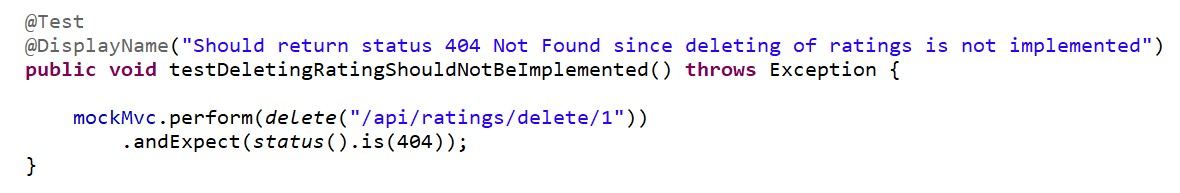
\includegraphics[width=0.6\textwidth]{slike/rating_controller_test.jpg}
				\caption{Testiranje brisanja komentara i ocjena}
				\label{fig:Testiranje brisanja komentara i ocjena}
			\end{figure}
			
			Sljedeća slika prikazuje da su se svi testovi uspješno proveli.
			\begin{figure}[h]
				\centering
				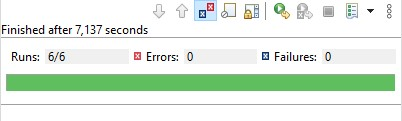
\includegraphics[width=0.6\textwidth]{slike/tests_passed.jpg}
				\caption{Uspješno provođenje testova}
				\label{fig:Uspješno provođenje testova}
			\end{figure}
			
			\subsection{Ispitivanje sustava}
			
			 Za ispitivanje sustava koristili smo alat Selenium WebDriver. Kako bi ga mogli koristit u projekt smo dodali  dependency za Selenium WebDriver. Također, bilo je potrebno i instalirati Chrome WebDriver.\newline
			 
			 \indent U prvom testu testirali smo dvije funkcionalnosti: dodavanje novog romobila i dodavanje oglasa za taj romobil. Korisnik se prvo prijavi u aplikaciju. S obzirom na to da su svi testovi započinjali s prijavom korisnika u aplikaciju, prijavu smo izdvojili u zasebnu funkciju. Koristeći objekt tipa WebDriver provjerili smo je li se korisnik uspješno prijavio u sustav te ako je, pozicionirali smo se na stranicu za pregled romobila. Da bi dodali novi romobil, bilo je potrebno unijeti sliku romobila i to smo učinili metodom sendKeys koju nudi WebDriver. Kliknuli smo na gumb za dodavanje romobila te provjerili je li se romobil uspješno dodao. Zatim smo kliknuli na gumb za dodavanje oglasa, ponovo metodom sendKeys unijeli sve zahtijevane informacije za dodavanje oglasa, dodali oglas i na kraju provjerili je li se oglas uspješno dodao. 
			 
			 \newpage
			 
			 \begin{figure}[h]
			 	\centering
			 	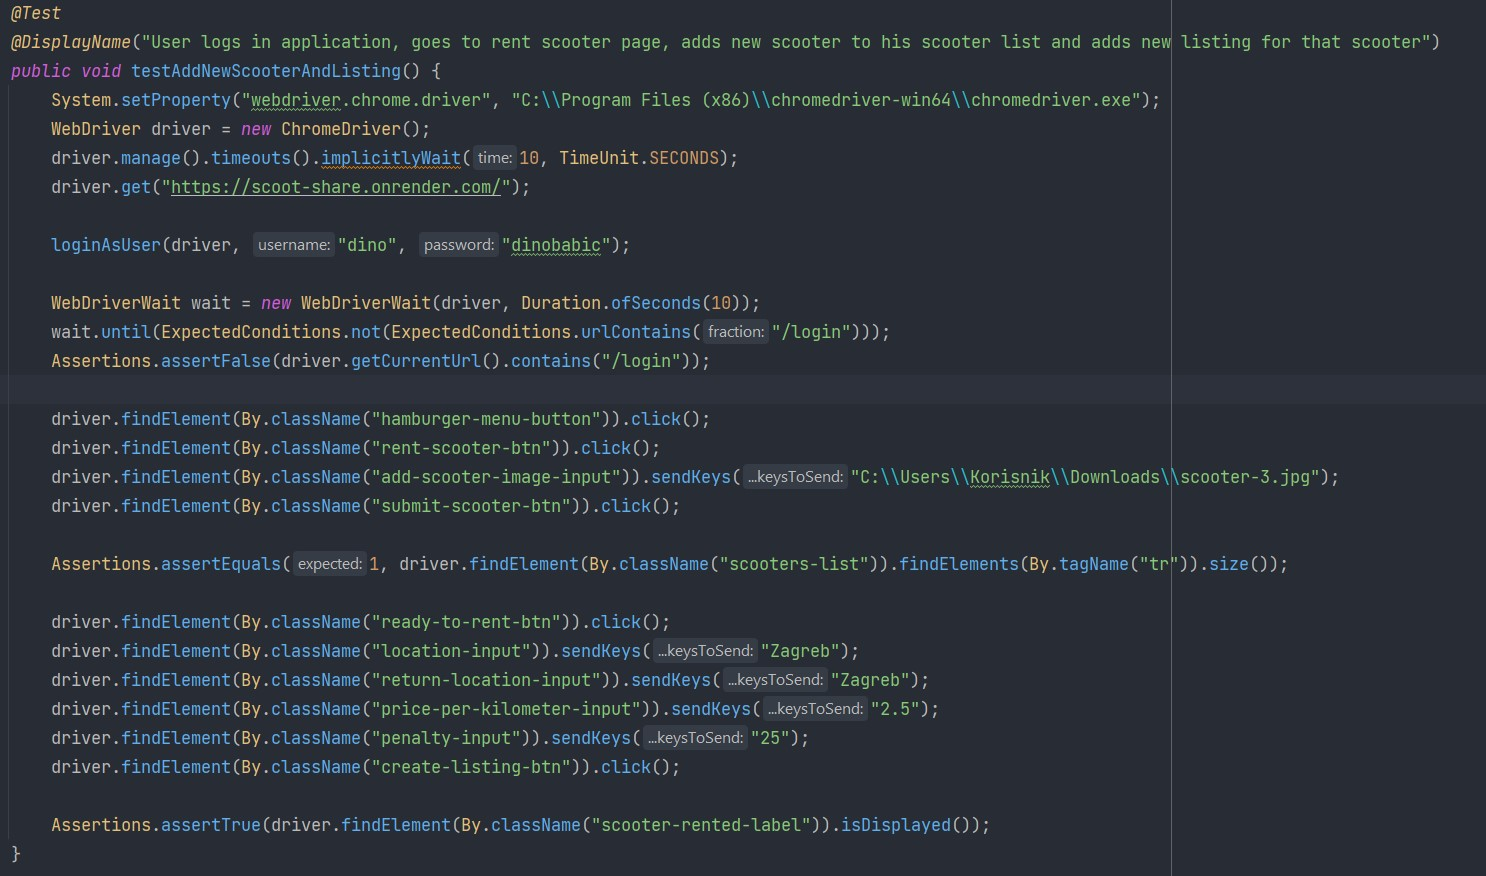
\includegraphics[width=0.6\textwidth]{slike/selenium_test_1.jpg}
			 	\caption{Testiranje dodavanja romobila i oglasa za romobil}
			 	\label{fig:Testiranje dodavanja romobila i oglasa za romobil}
			 \end{figure}
			 
			 \begin{figure}[h]
			 	\centering
			 	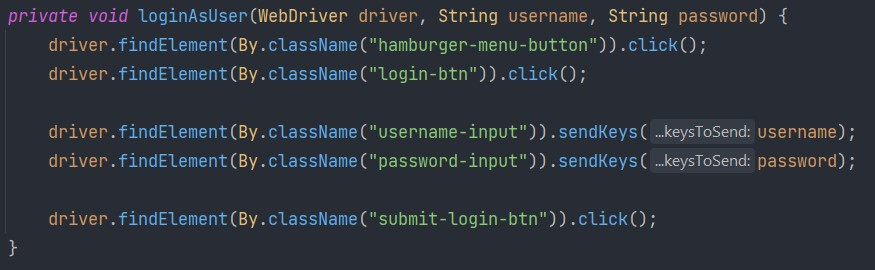
\includegraphics[width=0.6\textwidth]{slike/selenium_login.jpg}
			 	\caption{Funkcija za prijavu korisnika preko objekta tipa WebDriver}
			 	\label{fig:Funkcija za prijavu korisnika preko objekta tipa WebDriver}
			 \end{figure}
			 
			 
			 \indent U sljedećem testu provjerili smo mogućnost unajmljivanja romobila. Prijavili smo se u aplikaciju i odabrali smo prvi oglas na početnoj stranici. Očekivano ponašanje je da nas aplikacija usmjeri na stranicu koja prikazuje detalje o odabrano oglasu te smo to i testirali. Ako je ta provjera uspješno prošla, na stranici smo kliknuli gumb za unajmljivanje romobila. Testirali smo je li nas aplikacija preusmjerila  na stranicu s prikazom trenutno unajmljenih romobila i je li broj trenutno unajmljenih romobila jednak jedan.
			 
			 \begin{figure}[h]
			 	\centering
			 	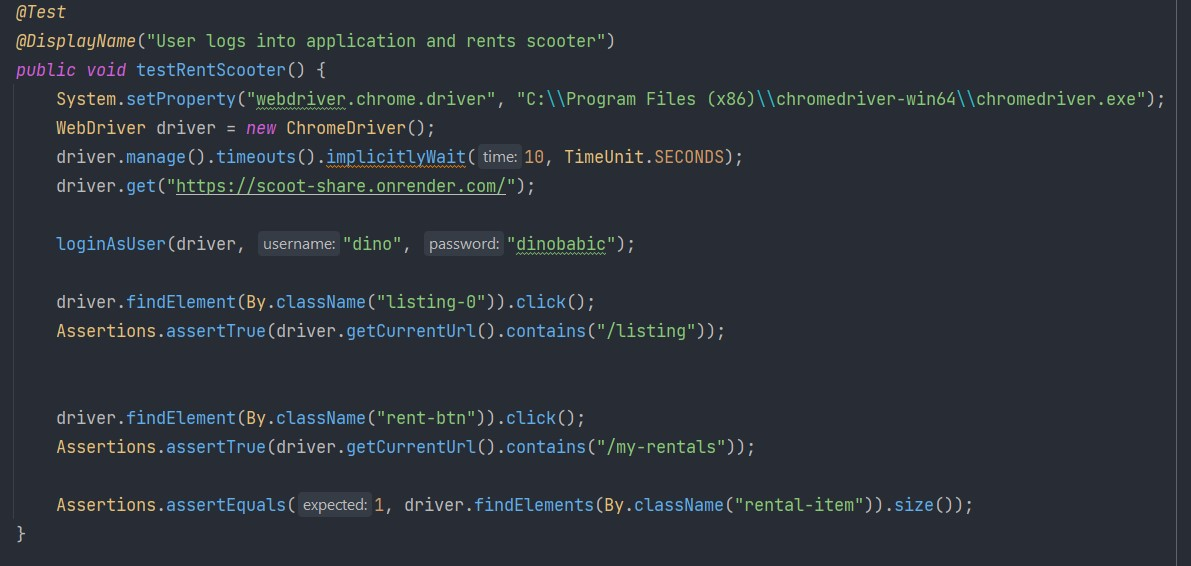
\includegraphics[width=0.7\textwidth]{slike/selenium_test_2.jpg}
			 	\caption{Testiranje unajmljivanja romobila}
			 	\label{fig:Testiranje unajmljivanja romobila}
			 \end{figure}
			 
			 \indent U posljednjem testu provjerili smo funkcionalnost dopisivanja između dva korisnika. Kreirali smo dva objekta tipa WebDriver, jedan za korisnika Dino i jedan za korisnika Marko. Prijavili smo oba korisnika u aplikaciju te smo ih koristeći njihove WebDriver objekte pozicionirali na stranicu za dopisivanje. Testirali smo je li početni broj poruka između ova dva korisnika jednak nuli. Nakon toga korinik Dino je poslao poruku korisniku Marko. S obzirom na to da je potrebno određeno vrijeme da poruka pristigne do Marka, pozvali smo Thread.sleep(500). Kada se dretva probudila, provjerili smo je li sada broj poruka jednak jedan. Slično smo ponovili još jednom, samo što je sada Marko slao poruku Dini.
			 
			 \begin{figure}
			 	\centering
			 	\subfigure{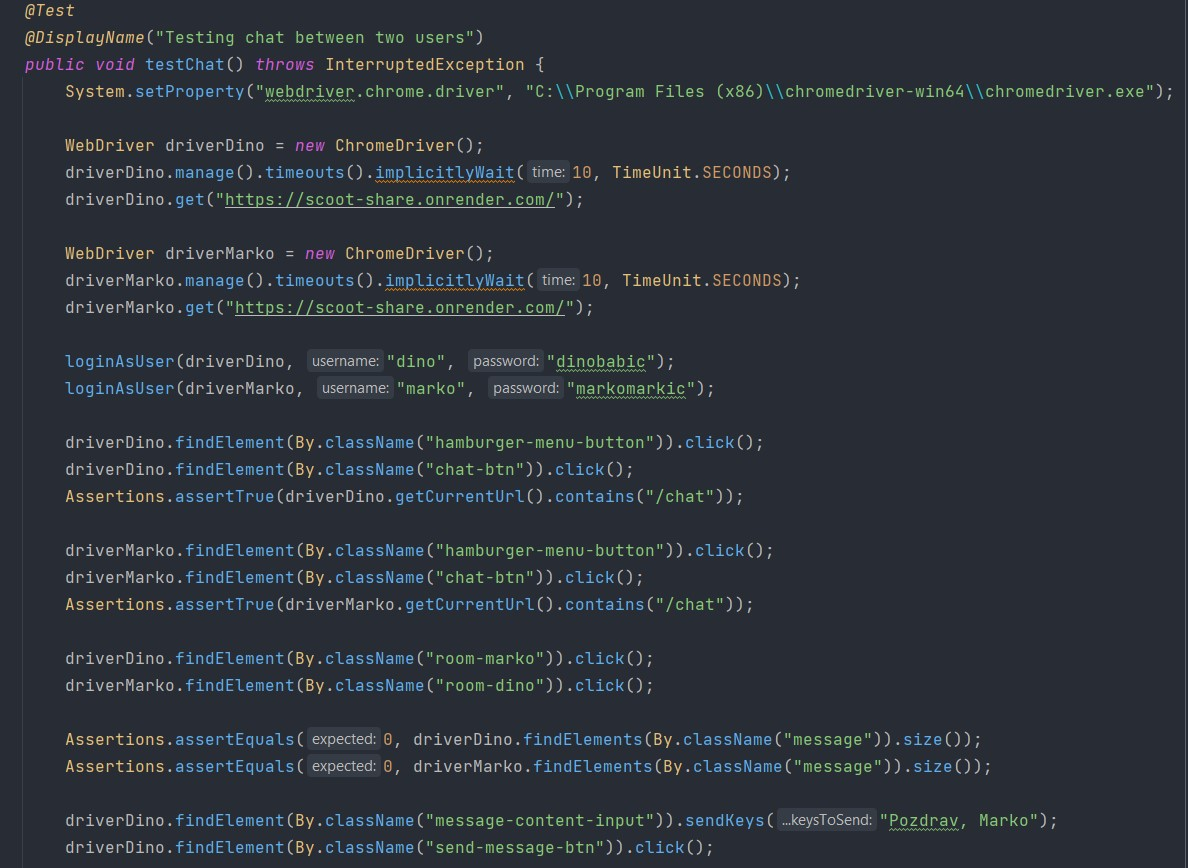
\includegraphics[width=0.7\textwidth]{slike/selenium_test_3_1.jpg}} 
			 	\subfigure{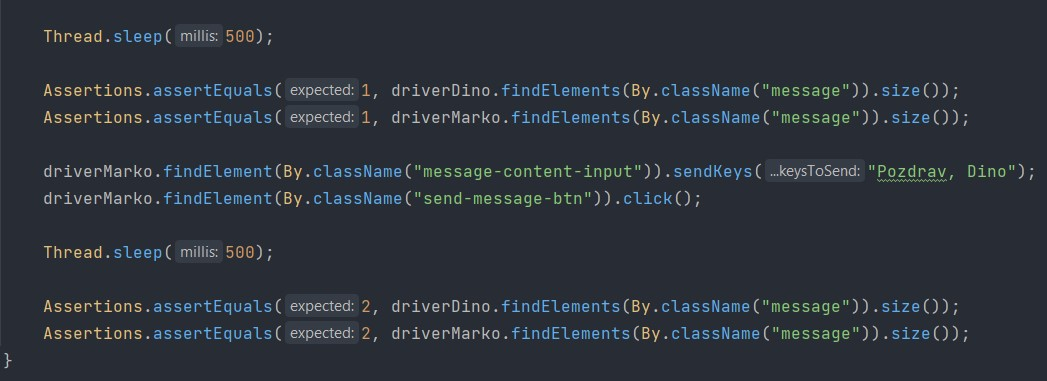
\includegraphics[width=0.7\textwidth]{slike/selenium_test_3_2.jpg}} 
			 	\caption{Testiranje razmjene poruka između korisnika}
			 	\label{fig:Testiranje razmjene poruka između korisnika}
			 \end{figure}
			 
		
		\newpage
		
		\section{Dijagram razmještaja}
			
			\textbf{\textit{dio 2. revizije}}
			
			 \textit{Potrebno je umetnuti \textbf{specifikacijski} dijagram razmještaja i opisati ga. Moguće je umjesto specifikacijskog dijagrama razmještaja umetnuti dijagram razmještaja instanci, pod uvjetom da taj dijagram bolje opisuje neki važniji dio sustava.}
			
			\eject 
		
		\section{Upute za puštanje u pogon}
		\indent Našu aplikaciju odlučili smo pustit u pogon preko platformue Render. U ovom poglavlju objasnit ćemo korake koje smo proveli kako bi uspješno pustili u pogon aplikaciju.\newline
	
		\textbf{Konfiguracija baze podataka}\newline
		Na web stranici Render potrebno je odabrati izradu nove baze podataka te unijeti željeno ime baze te verziju PostgreSQL-a. Sljedeća slika prikazuje izradu baze podataka.
		\begin{figure}[h]
			\centering
			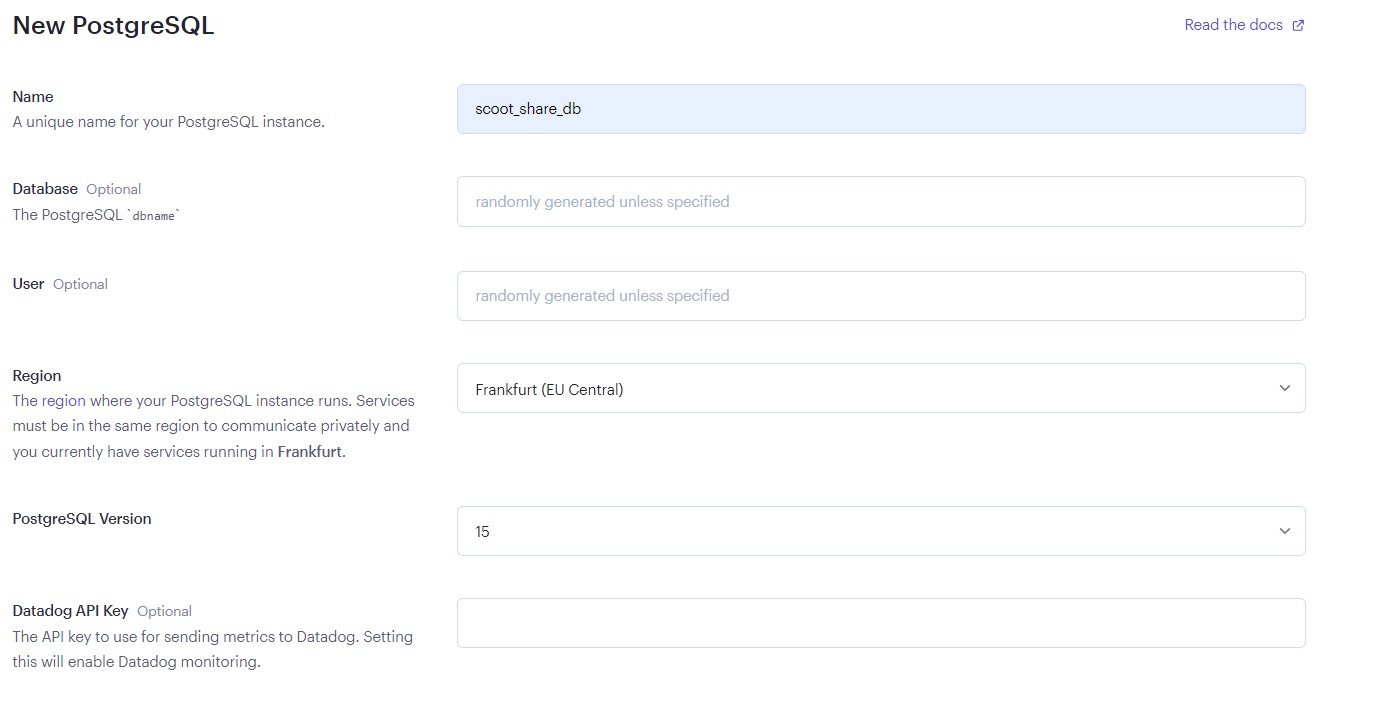
\includegraphics[width=0.8\textwidth]{slike/pustanju_u_pogon_1.jpg}
			\caption{Izrada baze podataka}
			\label{fig:baza podataka}
		\end{figure}
		
		
		\textbf{Konfiguracija backenda}\newline
		Kako bi mogli pustit u pogon našu poslužiteljsku stranu potrebno je učiniti određene izmjene. Potrebno je preurediti application.properties file na način da se dodaju globalne varijable koje će se koristit na Render-u. Također, treba dodati i Dockerfile koji sadrži niz instrukcija za izgradnju Docker kontejnera. 
		
		\begin{figure}
			\centering
			\subfigure{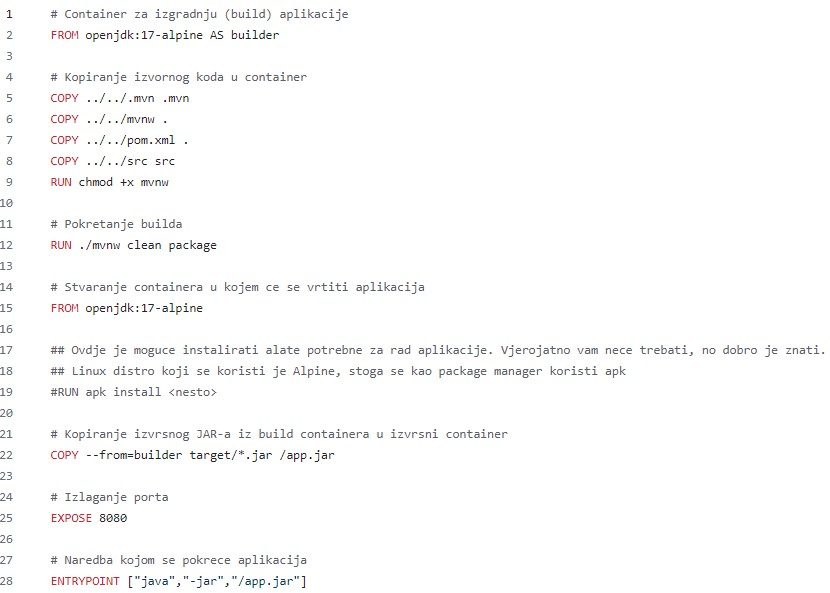
\includegraphics[width=0.24\textwidth]{slike/pustanju_u_pogon_2.jpg}} 
			\subfigure{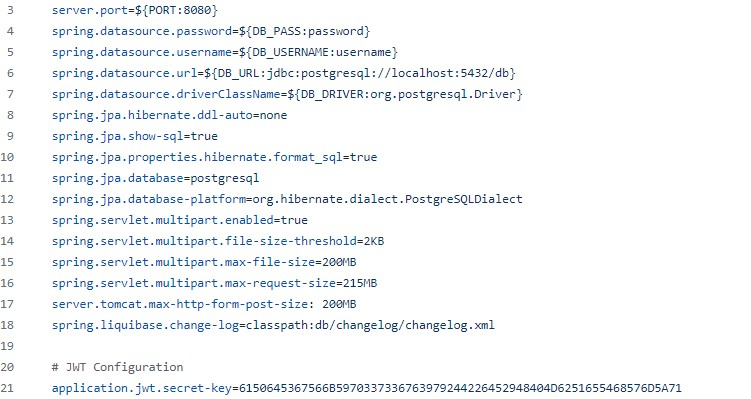
\includegraphics[width=0.24\textwidth]{slike/pustanju_u_pogon_3.jpg}} 
			\caption{Dockerfile i application.properties}
			\label{fig:dockerfile_application.properties}
		\end{figure}
		
		Nakon što je prvi korak odrađen potrebno je konfigurirati backend na Renderu. Odabiremo novi Web Service, nakon toga povežemo naš github repository s Renderom. 
		
		\begin{figure}[h]
			\centering
			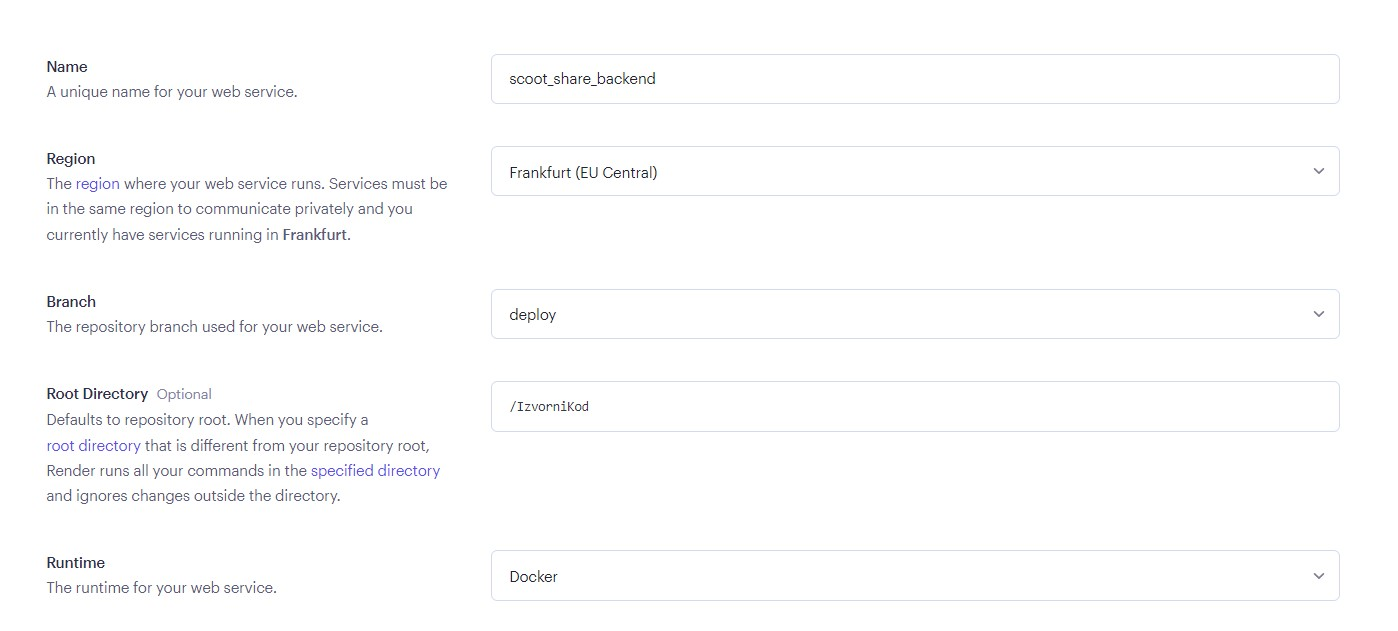
\includegraphics[width=0.8\textwidth]{slike/pustanju_u_pogon_4.jpg}
			\caption{Kreiranje backenda na Renderu}
			\label{fig:backend_render}
		\end{figure}
		
		\textbf{Konfiguracija frontenda}
		Potrebno je u našoj frontend React applikaciji u datoteci package.json dodati ovisnosti prema http-proxy-middleware, dotenv, express. Zatim treba dodati datoteku /src/setupProxy.js koja služi kao proxy server za lokalni development (redirecta api pozive na localhost:8080), odnosno kad se koristi react-scripts start skripta. Posljednja datoteka koju treba dodati je app.js u kojoj se nalazi express server za produkcijski proxy i posluzivanje frontenda. Jednom kada su sve izmjene napravljene i pohranjene u repozitorij kreirajmo Web Servis na Renderu za frontend. 
			
		\begin{figure}[h]
			\centering
			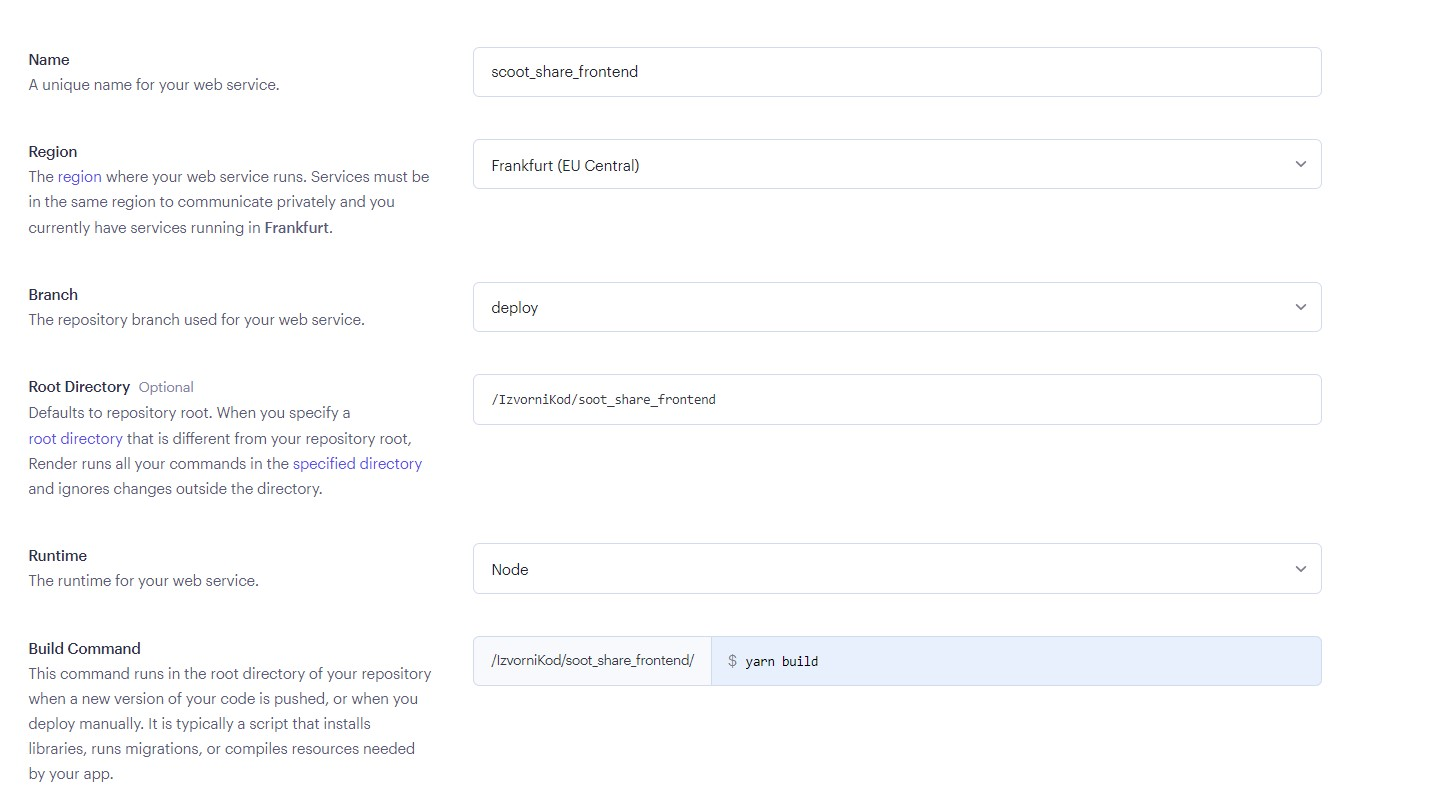
\includegraphics[width=0.8\textwidth]{slike/pustanju_u_pogon_5.jpg}
			\caption{Kreiranje frontenda na Renderu}
			\label{fig:frontend_render}
		\end{figure}
		
		Renderu će trebati jedno vrijeme da pokrene aplikacije te kada završi prikazat će URL adresu preko koje možemo pristupiti našoj aplikaciji. S obzirom da je Render nudi besplatno puštanje u pogon za očekivat je da će aplikacija raditi sporije, no za naše potrebe je to bilo sasvim dovoljno.
	\chapter{Zaključak i budući rad}
		
		\indent Zadatak naše grupe bila je izrada web aplikacije za iznajmljivanje romobila. Glavne funkcionalnosti aplikacije su pregled romobila, iznajmljivanje i unajmljivanje romobila. Tijekom čitavog semestra radili smo na razvoju projekta te smo nakon gotovo 15 tjedana projekt uspješno priveli kraju.\newline
		\indent U prvoj fazi projekta, naš tim se okupio radi razvoja aplikacije. Ovaj početni korak uključivao je dodjelu projektnog zadatka te usmjeren rad na dokumentiranje zahtjeva. Znali smo da će nam bez detaljnog i kvalitetnog dokumentiranja zahtjeva biti puno teže te smo zato ozbiljno pristupili tom dijelu. Tijekom ove faze, posvetili smo se izradi obrazaca uporabe, sekvencijskih dijagrama, modela baze podataka te dijagrama razreda. Ovi dokumenti pokazali su se ključnima prilikom suradnje s podtimovima odgovornim za razvoj backend-a i frontend-a. Vizualni prikazi idejnih rješenja problemskih zadataka, uključujući dijagrame i obrasce, pokazali su se izuzetno korisnima. Njihova izrada omogućila je jasno razumijevanje koncepta i uštedjela mnogo vremena tijekom drugog ciklusa razvoja, posebice kada su se pojavile nedoumice oko implementacije rješenja.\newline
		\indent U drugoj fazi projekta, fokus se pomaknuo prema implementaciji naše aplikacije. S progresijom rada na aplikaciji, suočavali smo se s naprednijim konceptima, što je zahtijevalo dodatno samostalno proučavanje alata i programskih jezika. Osim što smo aktivno radili na implementaciji aplikacije, bilo je nužno posvetiti se dokumentiranju preostalih zahtjeva i izradi potrebne popratne dokumentacije.Drugom fazom dominirala je intenzivna faza samostalnog rada gdje su članovi tima aktivno istraživali i primjenjivali stečena znanja u rješavanju izazova tehnološkog razvoja. Ovaj period samostalnosti pridonio je značajnom jačanju kompetencija tima, otvarajući put uspješnoj realizaciji postavljenih projektnih ciljeva. Ovaj intenzivan rad na razvoju aplikacije omogućio nam je dublje razumijevanje tehnoloških aspekata projekta.\newline
		\indent Korištenje videopoziva putem aplikacije Microsoft Teams pružilo nam je izvrsnu platformu za održavanje produktivnih sastanaka, olakšavajući fluidnu razmjenu informacija i znanja unutar tima.\newline
		\indent Za većinu članova tima ovo je bio prvi put da rade na razvoju aplikacije u timu, stoga je to izuzetno vrijedno iskustvo za sve nas. S obzirom da ćemo u budućnosti gotovo sigurno radit u timovima, drago nam je da smo se s tim načinom rada susreli već na faksu.Iako aplikacija ima svojih mana i mjesta za napredak, ponosni smo na postignuće koje smo ostvarili. 
	\chapter*{Popis literature}
		\addcontentsline{toc}{chapter}{Popis literature}
	 	
 		\textbf{\textit{Kontinuirano osvježavanje}}
	
		\textit{Popisati sve reference i literaturu koja je pomogla pri ostvarivanju projekta.}
		
		
		\begin{enumerate}
			
			
			\item  Programsko inženjerstvo, FER ZEMRIS, \url{http://www.fer.hr/predmet/proinz}
			
			\item  I. Sommerville, "Software engineering", 8th ed, Addison Wesley, 2007.
			
			\item  T.C.Lethbridge, R.Langaniere, "Object-Oriented Software Engineering", 2nd ed. McGraw-Hill, 2005.
			
			\item  I. Marsic, Software engineering book``, Department of Electrical and Computer Engineering, Rutgers University, \url{http://www.ece.rutgers.edu/~marsic/books/SE}
			
			\item  The Unified Modeling Language, \url{https://www.uml-diagrams.org/}
			
			\item  Astah Community, \url{http://astah.net/editions/uml-new}
		\end{enumerate}
		
		 
	
	
	\begingroup
	\renewcommand*\listfigurename{Indeks slika i dijagrama}
	%\renewcommand*\listtablename{Indeks tablica}
	%\let\clearpage\relax
	\listoffigures
	%\vspace{10mm}
	%\listoftables
	\endgroup
	\addcontentsline{toc}{chapter}{Indeks slika i dijagrama}


	
	\eject 
		
	\chapter*{Dodatak: Prikaz aktivnosti grupe}
		\addcontentsline{toc}{chapter}{Dodatak: Prikaz aktivnosti grupe}
		
		\section*{Dnevnik sastajanja}
		
		\begin{packed_enum}
			
			\item  sastanak
			\item[] \begin{packed_item}
				\item Datum: 20. listopada 2023.
				\item Prisustvovali: Anamarija Jakoubek, Dino Babić, Jan Grbac, Igor Šoštarko, Karemn Korić, Leonarda Pribanić, Ivan Pavelić
				\item Teme sastanka: Upoznavanje, Osnove projekta
				\begin{packed_item}
					\item Prvo upoznavanje, razmjenjivanje kontaktnih podataka i izrada skupne grupe.
					\item Biranje imena projekta, tehnologije koje će se koristiti, tko bi se kojim dijelom htio baviti te koliko ćemo se često sastajati.
				\end{packed_item}
			\end{packed_item}
			
			\item  sastanak
			\item[] \begin{packed_item}
				\item Datum: 24. listopada 2023.
				\item Prisustvovali: Anamarija Jakoubek, Dino Babić, Jan Grbac, Igor Šoštarko, Karemn Korić, Leonarda Pribanić, Ivan Pavelić
				\item Teme sastanka: Funkcionalni zahtjevi, Dijagrami, Arhitektura i Baza podataka
				\begin{packed_item}
					\item  Navođenje i razrada funkcionalnih i ostalih zahtjeva, koje će mogućnosti imati korisnici, a koji administratori
					\item  Razrađeni dijagrami i napravljene prve skice opisa obrazaca uporabe temeljene na funkcionalnim zahtjevima, također napisani prvi sekvencijski dijagrami koji opisuju kako će aplikacija funkcionirati u danim slučajevima
					\item Dogovor oko arhitekture klijent-poslužitelj koju ćemo koristiti kroz projekt. Za frontend je odabrana React, a za backend kombinacija Java, JavaScript i Spring Boot tehnologija. Prve skice baze podataka, tablica za entitete i postavljanje primarnih i stranih ključeva
				\end{packed_item}
			\end{packed_item}
			
			\item  sastanak
			\item[] \begin{packed_item}
				\item Datum: 7. studenog 2023.
				\item Prisustvovali: Anamarija Jakoubek, Dino Babić, Jan Grbac, Igor Šoštarko, Karemn Korić, Leonarda Pribanić, Ivan Pavelić
				\item Teme sastanka: Dijagrami razreda, Ažuriranje baze podataka
				\begin{packed_item}
					\item Crtanje dijagrama razreda, specifikacija metoda koje povlače Controller razred, definiranje entiteta i servisa koje će entiteti koristiti
					\item Dorada i ispravak baze podataka, dodavanje novih atributa u entitete ili cijele koji zamjenjuju nepotrebne funkcionalnosti baze podataka 
				\end{packed_item}
			\end{packed_item}
			
			\item  sastanak
			\item[] \begin{packed_item}
				\item Datum: 15. studenog 2023.
				\item Prisustvovali: Anamarija Jakoubek, Dino Babić, Jan Grbac, Igor Šoštarko, Karemn Korić, Leonarda Pribanić, Ivan Pavelić
				\item Teme sastanka: Dovršavanje prvog dijela dokumentacije, Objava i testiranje web-aplikacije
				\begin{packed_item}
					\item Ažuriranje slika, dijelova teksta, tablica i ostalih stavki prije prve predaje
					\item Deploy aplikacije na Render i testiranje funkcionalnosti prijave, registracije, odobravanje registracija i osnovnih funkcionalnosti web-stranice
				\end{packed_item}
			\end{packed_item}
			
			\item  sastanak
			\item[] \begin{packed_item}
				\item Datum: 20. studenog 2023.
				\item Prisustvovali: Anamarija Jakoubek, Dino Babić, Jan Grbac, Igor Šoštarko, Karemn Korić, Leonarda Pribanić, Ivan Pavelić
				\item Teme sastanka: Implementacija aplikacije
				\begin{packed_item}
					\item Ispravljanje grešaka u novim funkcionalnostima
					\item Podjela tima po funkcionalnostima koje je još potrebno implementirati
				\end{packed_item}
			\end{packed_item}
			
			\item  sastanak
			\item[] \begin{packed_item}
				\item Datum: 25. studenog 2023.
				\item Prisustvovali: Anamarija Jakoubek, Dino Babić, Jan Grbac, Igor Šoštarko, Karemn Korić, Leonarda Pribanić, Ivan Pavelić
				\item Teme sastanka: Dodavanje dijagrama u dokumentaciju
				\begin{packed_item}
					\item Dogovor oko izgleda dijagrama stanja, aktivnosti, razmještaja i komponenti
					\item Raspodjela tima za izradu dogovorenih dijagrama
				\end{packed_item}
			\end{packed_item}
			
			\item  sastanak
			\item[] \begin{packed_item}
				\item Datum: 10. prosinca 2023.
				\item Prisustvovali: Anamarija Jakoubek, Dino Babić, Jan Grbac, Igor Šoštarko, Karemn Korić, Leonarda Pribanić, Ivan Pavelić
				\item Teme sastanka: Ispitivanje rada sustava
				\begin{packed_item}
					\item Skupno testiranje funkcionalnosti sustava
					\item Stvaranje scenarija iz stvarnih primjera korištenja aplikacije
					\item Rješavanje problema na koje smo naišli tijekom testiranja
				\end{packed_item}
			\end{packed_item}
			
			\item  sastanak
			\item[] \begin{packed_item}
				\item Datum: 20. prosinca 2023.
				\item Prisustvovali: Anamarija Jakoubek, Dino Babić, Jan Grbac, Igor Šoštarko, Karemn Korić, Leonarda Pribanić, Ivan Pavelić
				\item Teme sastanka: Opisivanje instalacije i korištenja sustava
				\begin{packed_item}
					\item Opis instalacije i postavljanje sustava zajedno sa bazom podataka
					\item Opis procesa za klijentsko korištenje sustava
				\end{packed_item}
			\end{packed_item}
			
			\item  sastanak
			\item[] \begin{packed_item}
				\item Datum: 15. siječnja 2024.
				\item Prisustvovali: Anamarija Jakoubek, Dino Babić, Jan Grbac, Igor Šoštarko, Karemn Korić, Leonarda Pribanić, Ivan Pavelić
				\item Teme sastanka: Dovršavanje i ispravak dokumentacije
				\begin{packed_item}
					\item Dodavanje opisanih procesa u dokumentaciju, pisanje Zaključka i ideje za budući rad
					\item Ispravljanje pravopisnih grešaka, ažuriranje slika, dijagrama i tablica
				\end{packed_item}
			\end{packed_item}
			
			\item  sastanak
			\item[] \begin{packed_item}
				\item Datum: 16. siječnja 2024.
				\item Prisustvovali: Anamarija Jakoubek, Dino Babić, Jan Grbac, Igor Šoštarko, Karemn Korić, Leonarda Pribanić, Ivan Pavelić
				\item Teme sastanka: Ažuriranje aplikacije
				\begin{packed_item}
					\item Deploy nove verzije aplikacije na Render i testiranje cjelokupne funkcionalnosti sustava (prijava, registracija, iznajmljivanje i korištenje romobila, razmjena poruka, transakcije te ostavljanje ocjene i komentara)
				\end{packed_item}
			\end{packed_item}
			
			%
			
		\end{packed_enum}
		
		\eject
		\section*{Tablica aktivnosti}

			\begin{longtblr}[
					label=none,
				]{
					vlines,hlines,
					width = \textwidth,
					colspec={X[7, l]X[1, c]X[1, c]X[1, c]X[1, c]X[1, c]X[1, c]X[1, c]}, 
					vline{1} = {1}{text=\clap{}},
					hline{1} = {1}{text=\clap{}},
					rowhead = 1,
				} 
			
				\SetCell[c=1]{c}{} & \SetCell[c=1]{c}{\rotatebox{90}{\textbf{Ivan Pavelić}}} & \SetCell[c=1]{c}{\rotatebox{90}{\textbf{Jan Grbac}}} &	\SetCell[c=1]{c}{\rotatebox{90}{\textbf{Anamarija Jakoubek}}} & \SetCell[c=1]{c}{\rotatebox{90}{\textbf{Karmen Korić}}} &	\SetCell[c=1]{c}{\rotatebox{90}{\textbf{Dino Babić}}} & \SetCell[c=1]{c}{\rotatebox{90}{\textbf{Leonarda Pribanić}}} &	\SetCell[c=1]{c}{\rotatebox{90}{\textbf{Igor Šoštarko}}} \\  
				Upravljanje projektom 		& 5 & 3 &  &  & 4 &  & \\ 
				Opis projektnog zadatka 	&  &  & 2 & 5 &  &  & \\ 
				Funkcionalni zahtjevi       &  &  & 3 & 3 &  &  &  \\ 
				Opis pojedinih obrazaca 	&  &  & 1 & 4 &  &  &  \\ 
				Dijagram obrazaca 			& 4 & 4 & 4 &  & 4 & 4 & 4 \\ 
				Sekvencijski dijagrami 		& 2 & 2 & 2 &  & 2 & 2 & 2 \\ 
				Opis ostalih zahtjeva 		& 1 & 1 & 1 &  & 1 & 1 & 1 \\ 
				Arhitektura i dizajn sustava	&  &  &  &  &  & 3 & 4 \\ 
				Baza podataka				& 2 & 4 & 2 & 2 & 2 & 2 & 2 \\ 
				Dijagram razreda 			&  & 2 &  &  & 4 &  &  \\ 
				Dijagram stanja				&  &  & 1 & 1 &  & 1 &  \\ 
				Dijagram aktivnosti 		&  &  & 1 & 1 &  & 1 &  \\ 
				Dijagram komponenti			& 2 & 1 &  &  &  &  &  \\ 
				Korištene tehnologije i alati 		&  &  &  & 1 & 1 & 1 & 1 \\ 
				Ispitivanje programskog rješenja 	&  & 2 &  &  & 2 &  & 3 \\ 
				Dijagram razmještaja			& 1 & 2 &  &  &  &  &  \\ 
				Upute za puštanje u pogon 		& 1 &  & 2 &  &  & 1 &  \\  
				Dnevnik sastajanja 			& 1 &  &  & 1 &  & 1 &  \\ 
				Zaključak i budući rad 		&  &  & 2 & 1 & 2 &  &  \\  
				Popis literature 			& 1 & 1 &  &  & 1 &  & 1 \\  
				&  &  &  &  &  &  &  \\ \hline
				\textit{Izrada početne stranice} 	&  &  & 3 & 3 &  &  &  \\
				\textit{Frontend} 					&  &  & 6 & 6 & 7 &  &  \\    
				\textit{Izrada baze podataka} 		& 4 & 3 &  &  &  &  & 5\\  
				\textit{Spajanje s bazom podataka} 	& 3 & 2 &  &  &  & 4 & 3 \\ 
				\textit{Backend} 					& 2 & 5 &  &  & 5 & 3 & 2 \\ 
			\end{longtblr}
					
					
		\eject
		\section*{Dijagrami pregleda promjena}
		
		\begin{figure}[H]
			\centering
			
\includegraphics[width=0.8\textwidth]{slike/aktivnost.png}
			\caption{Prikaz aktivnosti na repozitoriju}
			\label{fig:your_label}
		\end{figure}
		
	


\end{document} %naredbe i tekst nakon ove naredbe ne ulaze u izgrađen dokument 


